\documentclass[12pt]{article}

\usepackage{notestyle}

\graphicspath{{./img/}}


\title{Appunti Database}
\author{Brendon Mendicino}



\begin{document}

\maketitle
\newpage
\tableofcontents
\newpage


\section{Introduzione}\label{sec:introduzione}


KDD: Knowledge Discovery from Data

\paragraph{Tecniche di data mining}
\begin{itemize}
    \item Regole di associazione: usate per trovare delle relazioni frequenti all'interno del database. Ad esempio: chi compra pannolini compra anche birra, il 2$\%$ degli scontrini contegono entrambe gli oggetti, il 30$\%$ degli scontrini che contengono pannalini contengono anche birra. Grazie alle regole di associazione si possono fare dei tipi di analisi come la basket analisys, ma puo essere utile anche per le raccomanadazioni.
    \item Classificazione: i classificatori predicono etichette discrete, esempio: nella posta elettronica alcune mail vengono segnate come spam. La classificazione definisce un modello per definire le predizioni, a volte non \`e sempre possibile creare dei modelli interpretabili ovvero dare una ragione per una determinata scelta.
    \item Clustering: gli algoritmi creano dei gruppi che raggruppano gli oggetti in esame, senza per\`o dare delle motivazioni delle scelte effettuate.
\end{itemize}





\section{Data Warehouse}
Un DW  \`e una base dati di supporto alla decisioni, che \`e mantenuta separatamente dalla base di dati operativa dell'azienda. I dati al suo interno sono:
\begin{itemize}
    \item orientati ai soggetti di interesse;
    \item integrati e consistenti;
    \item dipendenti dal tempo;
    \item non volatili;
    \item utilizzati per il supporto alle decisioni aziendali;
\end{itemize}


Per la progettazione concettuale di un DW, non esiste un formalismo universale, il modello ER non \`e adatto ma viene invece utilizzata il modello \textbf{Dimensional Fact Model}.

Il DFM \`e composto da:
\begin{itemize}
    \item Fatto: modella un insieme di eventi di interesse, che evolvono nel tempo (che pu\`o overe diversa granuralit\`a).
    \item Dimensioni: sono gli attribuiti di un fatto, generalmento sono categorici.
    \item Misure: discrive una caratteristica numerica di un fatto.
\end{itemize}
Sulle dimensioni si possono definire delle gerarachie, che definiscono di fatto una dipendenza funzionale tra gli attributi, quindi di 1 a n. Ad esempio: \textbf{data} ha un arco \textbf{mese}, una data ha uno ed un solo mese (1 a n).

I costrutti avanazati sono:
\begin{itemize}
    \item archi opzionali;
    \item dimensioni opzionali;
    \item attributo descrittivo: sono delle informazioni utili all'utente ma su cui non verteranno le interragazioni (ad esempio non si far\`a mai la group by su un indirizzo);
    \item non-additivit\`a: non si pu\`o fare la somma sulla metrica, il motivo \`e che non \`e modellato in modo tale da fare la somma;
\end{itemize}




\begin{itemize}
    \item Fatto: fenomeno di studio;
    \item Misure: attributi del fatto;
    \item Dimensioni: tabelle collegate al fatto;
\end{itemize}


\textbf{Schema a stella}:


\textbf{Snoflawke scheme}: si esplicitano le dipendenze funzionali, questo per\`o comporta un aumento delle operazioni di join.

Nella realt\`a lo snowflake \`e raramente utilizzato, il motivo \`e che il costo delle join pu\`o diventare oneroso. Un caso di utilizzo dello snowflake \`e quando si hanno dei dati condivisi.

\textbf{Archi multipli}:


\textbf{Dimensioni degeneri}: sono delle dimensioni con un solo attributo, questo si perch\`e nello stato attuale non si hanno delle specifiche per quell'attributo ma nel futuro si potrebbe facilmente estendere. Un'altra soluzione potrebbe essere un push down delle dimensioni degeri nella tabella dei fatti.

\textbf{Junk Dimension}: si pu\`o creare una dimensione che contenga tutte le dimensioni degeneri, le informazioni sono collegate semanticamente, \`e anche possibile unire delle informazioni scorrelate ma non \`e una scelta poco corretta, una soluzione potrebbe essere avere pi\`u junk dimensions.


\section{Analisi}
Sfruttando solo l'SQL \`e molto difficile fare delle analisi su un dw, infatti volendo calcolare delle operazioni per due argomenti diversi si devono fare pi\`u query. Estendendo il SQL si pu\`o, ad esempio, effettuare pi\`u operazioni leggendo una sola volta la tabella, ed effettuando il minor numero di join possibile.

\paragraph{Analisi OLAP}
I tipi di operazione sono:
\begin{itemize}
    \item roll up: riducendo il livello di dettaglio del dato, ovvero eliminare una o pi\`u clausole della groupby o navigare la gerarchia verso l'esterno;
    \item drill down: si aumenta il livello di dettaglio oppure si aggiunge una dimensione di analisi;
    \item slice and dice: consentono di ridurre il volume dei dati selezionando un sottogruppo dei dati di partenza;
    \item tabelle pivot: come viene mostrato il dato;
    \item ordinamento: ordinamento in base agli attributi;
\end{itemize}
Queste operazioni possono essere fatte con pi\`u o una query.

\subsection{Finestra di calcolo}
Una finestra di calcolo fa dei calcoli a partire da una query sottostante, la finestra ha 3 operazioni sottostanti:
\begin{itemize}
    \item partizionamento (\textbf{partition by}): partizionamnto dei dati, divide i record in gruppi a partire dall'attributo selezionato;
    \item ordinamento (\textbf{order by}): si definisce il criterio di ordinamento delle righe all'interno dei partizionamenti;
    \item finestra di aggregazione (\textbf{over}): porzione di dati, specifica per ogni riga di dato, su cui effettuare dei calcoli;
\end{itemize}
\begin{example}{}{}
    Data la tabella Vendite(\underline{Citt\`a}, \underline{Mese}, Importo), calcolare per ogni citt\`a la media delle vendite per il mese corrente ed i due precedenti.

\begin{lstlisting}[language=sql]
SELECT Citta, Mese, Importo,
    AVG(Importo) OVER (PARTITION BY Citta)
                        ORDER BY Mese
                        ROWS 2 PRECEDING)
    AS MediaMobile
FROM Vendite;
\end{lstlisting}
\end{example}
Quando la finestra \`e incompleta il calcolo \`e effettuato sulla parte presente, \`e possibile specificare che se la riga non \`e presente il risultato deve essere NULL.

Si pu\`o definire un intervallo fisico, superiore o inferiore. 
\begin{lstlisting}[language=sql]
    ROWS BETWEEN 1 PRECEDING AND 1 FOLLOWING
\end{lstlisting}
\`E possibile definire la tupla currente e quella che la precedono e che la seguono
\begin{lstlisting}[language=sql]
ROWS UNBOUNDED PRECEDING (o FOLLOWING)
\end{lstlisting}
Il rggruppamento fisico \`e specifico per quando i dati non hanno delle interruzioni.


Per definire un intervallo logico si utilizza il costrutto \textbf{range}.

\begin{lstlisting}[language=SQL]
SELECT Citta, Mese, Importo,
    Importo / SUM(Importo) OVER () AS PerOverMax,
    Importo / SUM(Importo) OVER (PARTITION BY Citta) AS PerOverCity,
    Importo / SUM(Importo) OVER (PARTITION BY Mese) AS PerOverMonth
FROM Vendite
\end{lstlisting}


Se una \textbf{group by} \`e presente all'interno della query allora, tutte le entry che possono comparire nella finestra di calcolo sono solo quelle che compaiono nella group by.

\paragraph{Funzione di ranking}
La funzione di ranking serve a creare delle classifiche

\begin{itemize}
    \item \textbf{rank()}: la funzione rank in presenza di pi\`u oggetti nella stessa posizione salta al prossimo record;
    \item \textbf{denserank()}: la funzione denserank tiene tutte righe con la stessa posizione;
\end{itemize}

...
\begin{lstlisting}[language=sql]
SELECT Citta, Mese, SUM(Importo) AS TotMese,
    RANK() OVER (PARTITION BY Citta
                ORDER BY SUM(Import) DESC)

FROM Vendite, ...
WHERE ...
GROUP BY Citta, Mese
\end{lstlisting}



\paragraph{Estensione della group by}
\begin{itemize}
    \item \textbf{rollup}: consente di calcolare le aggragazioni su tutti i possibili gruppi, eliminando una colonna alla volta, da destra verso sinistra, esempio: calcola le vendite per: (Citta, Mese, Prodotto), (Citta, Mese), (Citta):
        \begin{lstlisting}[language=sql]
SELECT Citta, Mese, Prodotto, SUM(Importo) AS TotVendite
FROM ...
WHERE ...
GROUP BY ROLLUP (Citta, Mese, Prodotto)
        \end{lstlisting}
    \item \textbf{cube}: consente di calcolare tutte le possibili combinazioni del ragrruppamento;
    \item \textbf{grouping sets}: serve a definire degli aggregati su gruppi specifici definiti dall'utente;
\end{itemize}


\subsection{Sintassi ORACLE}
Raggruppamento fisico:
\begin{example}{}{}
    Selezionare, separatamente per ogni citt\`a, per ogni data l'importo e la media dell'importo dei due giorni precedenti.
    \begin{lstlisting}[language=sql]
select citta, data, importo,
    avg(importo) over (partition by citta
                        order by data
                        rows 2 preceding
    ) as mediaMobile
from vendite
order by citta, data;
    \end{lstlisting}
\end{example}


Raggruppamento logico:
\begin{example}{}{}
   \begin{lstlisting}[language=sql]
select citta, data, importo,
    avg(importo) over (PARTITION BY citta
                        ORDER BY data
                        RANGE BETWEEN INTERVAL '2'
                        DAY PRECEDING AND CURRENT ROW
    ) as mediaUltimi3Giorni
from vendite
order by citta, data;
   \end{lstlisting}
\end{example}

\begin{example}{}{}
    \begin{lstlisting}[language=sql]
select COD_A, sum(Q) as sommaPerArticolo,
    rank() over (order by sum(Q) desc) as graduatoria
from FAP
group by COD_A
    \end{lstlisting}
\end{example}


All'interno di oracle sono preseti delle funzionalit\`a aggiuntive oltre alla funzione di rank, come: 

\paragraph{ROW\_NUMBER}
Assegno un numero progressivo ad ogni elemento in una partizione.

\begin{lstlisting}[language=sql]
select tipo, peso,
    row_number over (partition by tipo
                    order by tipo)
from ...
where ...;
\end{lstlisting}

\paragraph{CUME\_DIST}
Consente di calcolare le distribuzine cumulativa all'interno di una partizione, permette di definire un valore sulla distribuzione dei valori.


\paragraph{NTILE(n)}
Una funzione che da la possibilit\`a di dividere le partizioni in sottogruppi
\begin{lstlisting}[language=sql]
select tipo, perso, 
    ntile(3) over (partition by tipo order by peso) as ntile3peso
from ...
where ...;
\end{lstlisting}



\subsection{Esercizi}
Cliente(CodCliente, Cliente, Provincia, Regione) \\
Categoria(CodCat, Categoria) \\
Agente(CodAgente, Agente, Agenzia) \\
Tempo(CodTempo, Mese, Trimestre, Semestre, Anno) \\
Fatturato(CodTempo, CodCliente, CodCatArticolo, CodAgente, TotFatturato, NumArticoli, TotSconto) 

\vspace{.8cm}

1. Visualizzare per ogni categoria di articoli
\begin{itemize}
    \item la categoria
    \item la quantità totale fatturata per la categoria in esame
    \item il fatturato totale associato alla categoria in esame
    \item il rank della categoria in funzione della quantità totale fatturata
    \item il rank della categoria in funzione del fatturato totale
\end{itemize}
\begin{lstlisting}[language=sql]
select categoria, sum(numArticoli),
    sum(totFatturato),
    rank() over (order by sum(numArticoli) desc),
    rank() over (order by sum(totFatturato) desc)
from fatturato f, categoria c
where f.codCatArticolo = c.codCat
group by categoria;
\end{lstlisting}
2. Visualizzare per ogni provincia
\begin{itemize}
    \item la provincia
    \item la regione della provincia
    \item il fatturato totale associato alla provincia
    \item il rank della provincia in funzione del fatturato totale, separato per regione
\end{itemize}
\begin{lstlisting}[language=sql]
select provincia, regione,
    sum(totFatturato) as fatturatoPerProvincia,
    rank() over (partion by regione
                 order by sum(totFatturato) desc
    ) as rankFatturatoPerRegione
from cliente c, fatturato f
where c.codCliente = f.codCliente
group by provincia, regione;
\end{lstlisting}
3. Visualizzare per ogni provincia e mese
\begin{itemize}
    \item la provincia
    \item la regione della provincia
    \item il mese
    \item il fatturato totale associato alla provincia nel mese in esame
    \item il rank della provincia in funzione del fatturato totale, separato per mese
\end{itemize}
\begin{lstlisting}[language=sql]
select provincia, regione, mese,
    sum(totFatturato) as fatturatoPerProvinciaPerMese,
    rank() over (partition by mese
                order by sum(totFatturato)
    ) as rankFatturatoPerMese
from cliente c, fatturato f, tempo t
where c.codCliente = f.codCliente and t.codTempo = f.codTempo
group by provincia, regione, mese;
\end{lstlisting}
4. Visualizzare per ogni regione e mese
\begin{itemize}
    \item la regione
    \item il mese
    \item il fatturato totale associato alla regione nel mese in esame
    \item l’incasso cumulativo al trascorrere dei mesi, separato per ogni regione
    \item l’incasso cumulativo al trascorrere dei mesi, separato per ogni anno e regione
\end{itemize}
\begin{lstlisting}[language=sql]
select regione, mese,
    sum(TotFatturato) as fatturatoPerMese,
    sum(TotFatturato) over (
        partition by regione
        order by mese
        rows unbounde preceding
    ) as incassoCumulativoTot,
    sum(TotFatturato) over (
        partition by regione, anno
        order by mese
        rows unbounded preceding
    ) as incassoCumulativoPerAnno
from cliente c, fatturato f, tempo t
where c.CodCliente = f.CodCliente and t.CodTempo = f.CodTempo
group by regione, mese, anno;
\end{lstlisting}



\newpage
\section{Viste materializzate}
Le viste materializzate sono necessarie per ridurre la lentezza della operazioni di group by per grandi moli di dati, le viste materializzate sono dei sommari precalcolati della tabella dei fatti.

Le VM usano con con costruto pricipale la group by, quando si crea una VM \`e convienente includere anche le dimensioni a granularit\`a superiori, in modo da poter riutilizzare la tabella.

Per rappresetnare le dipendenze delle viste materializzate si utilizza un \textbf{reticolo multidimensionale}. Pi\`u ci si trova in alto al reticolo pi\`u ci si avvina alle dimensioni della tabella dei fatti, pi\`u si va in basso pi\`u si trova un granuralit\`a maggiore.

La scelta delle viste viste tra tutte le possibili combinazioni \`e data da:
\begin{itemize}
    \item si scelgie una sola vista da cui \`e possibile raggiungere tutti gli attributi;
    \item creo una vista per ogni query;
    \item scelgo delle viste intermedie che possono portare a ripsondere e pi\`u query;
\end{itemize}

\subsection{Documentazione Oracle}
Riducono i tempi di esecuzione delle group by e non si eseguono pi\`u le join. Nel DBMS Oracle esiste la \textbf{query rewriting}, che permette grazie all'ottimizzatore di interpretare le query e se i risultati corrispondono alle condizioni di creazioni delle viste, allora le query viene riscritta con la vista.
\begin{lstlisting}[language=sql]
create materialized view NAME
[build {immediate|deferred}]
[refresh {complete|fast|force|never}
         {on commit|on demand}]
[enable query rewrite]
as
    QUERY
\end{lstlisting}
\begin{itemize}
    \item immediate: lo schema della tabella viene popolata immediatamente, dato dallo schema di attributi presenti nella select;
    \item deferred: la vista viene creata, ma viene popolata successivamente;
    \item complete: i dati vengono presi interamente dal database;
    \item fast: i dati vengono presi in modo incrementale;
    \item force: se possibile viene eseguito il refresh in modalit\`a fast, oppure in modalit\`a complete;
    \item never: la vista non viene mai aggiornata;
    \item on commit: ogni volta che viene fatto un commit sulla tabella della query anche la vista viene aggiornata;
    \item on demand: viene definito dall'utente quando aggiornare la vista;
    \item enable query rewrite: abilita il dbms ad usare la vista per accellerary le query;
\end{itemize}
Quando si ha bisogno del \textbf{fast refresh}, la vista meterializzata ha bisogno di informazioni aggiuntive, che vengono fornita da tabella di log che informano delle nuove operazioni (insert, delete, update) effettuate sul db, la \textbf{materialized view log} \`e associata ad una tabella che ha subito delle variazioni:
\begin{lstlisting}[language=sql]
create materialized view log on TABELLA
with sequence, rowid
(COLONNA, ...)
including new values;
\end{lstlisting}
\begin{itemize}
    \item squence: istante temporale in cui \`e avvenuta la modifica;
    \item rowid: indica la tupla che ha subito una modifiche;
\end{itemize}
Su queste keyword si deve difinire una lista di attributi da monitorare, si aggiunge \textbf{including new values} per supportare l'inserimento di nuove tuple.

Per poter usare insieme l'opzione \textbf{fast refresh}, il log deve essere creato su tutte le colonne utilizzate all'interno della query della vista meterializzata, esempio:
\begin{lstlisting}[language=sql]
CREATE MATERIALIZED VIEW VIEW1
BUILD IMMEDIATE
REFRESH FAST ON COMMIT
ENABLE QUERY REWRITE
AS
    SELECT
        TRI,
        SEM,
        ANNO,
        SETTORE,
        UNIVERISTA,
        STATO,
        SUM(NUM_PUBBLICAZIONI)
    FROM
        PUBBLICAZIONI P,
        AUTORE_MAIN   A,
        DATA          D
    WHERE
        P.IDDATA = D.IDDATA
        AND P.IDAUTORE = A.IDAUTORE
    GROUP BY
        TRI,
        SEM,
        ANNO,
        SETTORE,
        UNIVERSITA,
        STATO;

-- logs
CREATE MATERIALIZED VIEW LOG ON DATA WITH ROWID,
SEQUENCE (
    IDDATA,
    TRI,
    SEM,
    ANNO
) INCLUDING NEW VALUES;

CREATE MATERIALIZED VIEW LOG ON AUTORE_MAIN WITH ROWID,
SEQUENCE (
    IDAUTORE,
    SETTORE,
    UNIVERSITA,
    STATO
) INCLUDING NEW VALUES;

CREATE MATERIALIZED VIEW LOG ON PUBBLICAZIONI WITH ROWID,
SEQUENCE (
    IDDATA,
    IDLOUGO,
    IDAUTORE,
    NUM_PUBBLICAZIONI
) INCLUDING NEW VALUES;
\end{lstlisting}





\newpage
\section{Alimentazione dei Data Warehouse}
Essendo dei dati derivati, la prima operazione da effettuare \`e l'ETL, se questo \`e complesso si va a definire un area di staging in cui il dato viene matenuto temporaneamente. Il processo di ETL va gestito sei per il popolamento del DW sia per quando verr\`a aggiornato con dati nuovi.

\subsection{Estrazione}
L'estrazione statica \`e la prima estrazione effettuata per popolare il DW. Per fare l'estrazione incrementale si possono:
\begin{itemize}
    \item creare delle applicazioni ad hoc per i sistemi legacy;
    \item usando dei log, che non vanno ad interferire con il carico del db;
    \item usando dei trigger: sono proceddure che si attivano quando degli si effettuano delle operazioni specifiche;
    \item basata su timestamp: dove i recordi hanno il timestamp dell'ultima modifica effettuata su di essi;
\end{itemize}

\subsection{Pulitura}
Quando si effettua una estrazione ci si potrebbe trovare di fronte a:
\begin{itemize}
    \item dati duplicati;
    \item dati mancanti;
    \item campo non previsto;
    \item valori errati o impossibili;
    \item inconsistenza del valore;
\end{itemize}
Ogni errore richede una tecnica specifica per essere risolto, le pi\`u comuni sono l'uso di dizionari per controllare errori di battitura, oppure il \textbf{join approssimato}, ad esempio: due database non hanno una chiave condivisa per identificare un utente dall'ordine effettutato, allora per fare una join si dovranno prendere i campi comuni, controllandone sempre la consistenza, oppure i problemi di \textbf{merge/purge}, ad esmpio: facendo il merge di due db le informazioni potrebbero essere duplicate ...

\subsection{Trasformazione}
Conversione dei dati nel formato di quelli presenti nel data warehouse.

\subsection{Caricamento}
In fase di caricamento i dati si caricano nel seguente ordine:
\begin{itemize}
    \item dimensioni;
    \item fatti;
    \item indici e viste;
\end{itemize}




\begin{problem}{Progettazione Magazzini}{progettazione-magazzini}
    \hbadness=99999
    Tabelle: \\
    Tempo(\underline{codT}, data, mese, 3m, 4m, 6m, anno) \\
    Magazzino(\underline{codMa}, magazzino, citta, provincia, regione) \\
    Modello(\underline{codMo}, modello, categoria) \\
    \texttt{UsoMtqMagazzino(\underline{codMa}, \underline{codT}, mtqLiberi, mtqTot) \\
    UsoProdMagazzino(\underline{codMa}, \underline{codMo}, \underline{codT}, numeroProdottiTotale, valoreTotaleProdotii) }

    Query:
    \begin{enumerate}
        \item Relativamente al primo trimestre dell’anno 2013, considerando solo i magazzini della città di Torino,trovare per ogni coppia (magazzino,data) il valore complessivo di prodotti presenti in tale data nelmagazzino e il valore complessivo medio giornaliero di prodotti presenti nel magazzino nel corsodella settimana precedente la data in esame (data in esame inclusa):
\begin{lstlisting}[language=sql]
select magazzino, data,
    sum(valoreTotProdotti) as valoreTot,
    avg(sum(valoreTotProdotti)) over (
        partition by magazzino
        order by data
        range between interval '7'
        day preceding and current row
    ) as valoreMedioSuGiornoCorrenteESettimanaPrecedente

from UsoProdMagazzino u, Tempo t, Magazzino m
where u.codT = t.codT and
    u.codMa = m.codMa and
    citta = 'torino' and
    anno = 2013 and
    3m = 1
group by magazzino, data;
\end{lstlisting}
        \item Relativamente all’anno 2004, trovare per ogni coppia(città,data) la percentuale di superficie liberagiornaliera nella città. Associare ad ogni coppia un attributo di rank legato alla percentuale disuperficie libera giornaliera nella città (1 per la coppia con la più bassa percentuale di superficielibera giornaliera).
\begin{lstlisting}[language=sql]
select citta, data,
    sum(mtqLiberi) / sum(mtqTot) * 100 as percentualeMtqLiberi,
    rank() over (
        order by sum(mtqLiberi) / sum(mtqTot) * 100
    ) as rankLowestPercentuale
from Tempo t, Magazzino m, UsoMtqMagazzino u
where t.codT = u.codT and
    m.codMa = u.codMa and
    anno = 2004
group by citta, data;
\end{lstlisting}
        \item Relativamente ai primi sei mesi dell’anno 2014, trovare per ogni coppia (magazzino,data) la percentuale di superficie libera giornaliera.
\begin{lstlisting}[language=sql]
select magazzino, data,
    100 * sum(mtqLiberi) / sum(mtqTot) as percentualeMtqLiberi
from Tempo t, Magazzino m, UsoMtqMagazzino u
where t.codT = u.codT and
    m.codMa = u.codMa and
    anno = 2014 and
    mese <= 6
group by magazzino, data;
\end{lstlisting}
        \item Relativamente all’anno 2013, trovare per ogni coppia (magazzino,mese) il valore complessivo medio giornaliero di prodotti presenti.
\begin{lstlisting}[language=sql]
select distinct magazzino, mese,
    avg(sum(valoreTotProdotti)) over (
        parition by magazzino, mese
    ) as valoreMedioGiornalieroComplessivo
from UsoProdMagazzino u, Tempo t, Magazzino m
where u.codMa = m.codMa and
    u.codT = t.codT and
    anno = 2013
group by magazzino, mese, data;
\end{lstlisting}
        \item Relativamente all’anno 2015, trovare per ogni regione il valore complessivo medio giornaliero di prodotti presenti nella regione.
\begin{lstlisting}[language=sql]
select regione, mese,
    avg(sum(valoreTotProdotti)) over (
        parition by regione, mese
    ) as valoreMedioGiornalieroComplessivo
from UsoProdMagazzino u, Tempo t, Magazzino m
where u.codMa = m.codMa and
    u.codT = t.codT and
    anno = 2015
group by regione, mese, data;
\end{lstlisting}
        \item Relativamente all’anno 2014, trovare per ogni coppia(mese, regione) la percentuale di superficie libera giornaliera nella regione.
\begin{lstlisting}[language=sql]
select regione, mese,
    avg (100 * sum(mtqLiberi) / sum(mtqTot)) over (
        partition by regione
    )
from UsoMtqMagazzino u, Tempo t, Magazino m
where u.codMa = m.codMa and
    u.codT = t.codT and
    anno = 2014
group by regione, mese, data;
\end{lstlisting}
    \end{enumerate}
\end{problem}




\section{Data Lake}
I data lake sono dei repositori di dati, storicizzati per utilizzo futuro cos\`i come sono disponibili, in qualsiasi formato. Questi raw data potrebbero essere utilizzati in futuro.

I data lake danno la possibilit\`a di storicizzare i dati per un uso futuro, inoltre tutti i dati sono contunuti in un repository comune, infatti \`e caratterizzato da bassi costi di storage e mantenimento, per\`o pu\`o essere difficile estrapolare dei dati.

\newpage
\section{Data processing}
Una collezione \`e costituita da oggetti di dato,
\begin{itemize}
    \item \textbf{Attributo}: \`e una propriet\`a dell'oggetto;
    \item \textbf{Tipi di Attributo}: possono essere nominali, ordinali, intervalli, rapporti;
    \item \textbf{Proprit\`a dei valori degli attributi}: possiamo definire equivalenza, ordine, addizione, moltiplicazione;
    \item \textbf{Attributi discreti e continui}:  discreti hanno un nemero finito di valori, i continui hanno dei valori reali;
\end{itemize}

Tipi di dato da analizzare:
\begin{itemize}
    \item record: sono i dati presenti in una tabella;
    \item grafi: come la struttura di una pagina web;
    \item ordinato: dati in cui esiste il concetto di squenza;
\end{itemize}

Esistono vari tipi di dato:
\begin{itemize}
    \item \textbf{Document Data} Per ogni riga ho un doumento, per ogni colonna ho degli attributi che descrivono delle parole chivi all'interno del documento, ogni riga \`e un array che contiene la pesatura degli attributi, la pesatura pu\`o essre calcolata con algoritmi specifici;
    \item \textbf{Dato transazionale} Un dato transazionale \`e formato da un insieme di items all'interno della tabella, ogni transazione \`e identificata da un ID, nelle tabelle transazionali non esiste il concetto di ordine ne tra le riche, ne all'interno della transazione;
    \item \textbf{Dato a grafo}: ad esempio le pagine web hanno dei link ad altre pagine, potrei considere i link come gli archi del grafo, ognuno con un peso specifico, e la singola pagina come un nodo del grafo;
    \item \textbf{Qualit\`a del dato}: nella maggior parte dei casi i dati presentano delgi errori, questi possono essere causati da rumori e outliers, dati mancanti o duplica, ...;
    \item \textbf{Outliers}: dati che escono al di fuori del comportamento medio e quindi molto rumorosi, l'abbiettivo dell'analisi di outlier detection \`e l'individuazione di questi dati e dell'eliminazione;
\end{itemize}




\subsection{Data preprocessing}
Le tecniche di preprocessing sono:
\begin{itemize}
    \item \textbf{data aggregation}: Consente di combinare pi\`u record o pi\`u attributi, si fa questo per effettuare una riduzione della quantit\`a di dati, ed avere dei dati pi\`u stabili con una vairiabilit\`a minore.
    \item \textbf{data reduction}: Si possono effetuare due tipi di riduzione: riduzione degli attributi o riduzione dei valori. Per effettuare queste riduzioni esistono delle tecniche specifiche.
\end{itemize}
Un altra tecnica di data preprocessing \`e il \textbf{sampling} \`e una tecnica di statistica di analisi, ad esempio nella pipeline di datascience il sampling serve per trovare delle rappresentazioni adatte al dataset, facendo N esperimenti su un sample preso dal dataset si andranno a fare dei test sull'intero dataset per verificare che le ipotesi siano confermate, in figura si pu\`o vedere come il grafico col numero pi\`u piccolo di campia non sia pi\`u rappresentativo del dataset originale.
\begin{figure}[H]
    \centering
    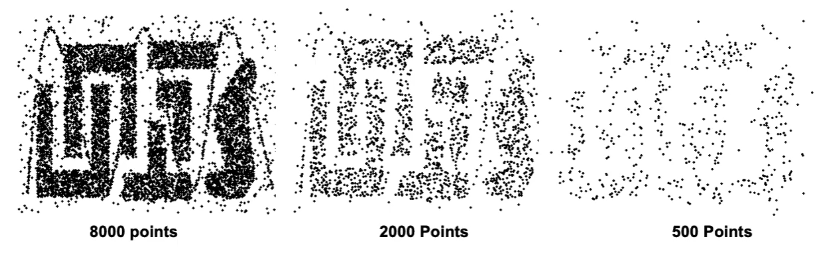
\includegraphics[width=0.8\textwidth]{sampling-example.png}
    \caption{Sampling Example}
    \label{fig:sampling-example}
\end{figure}
I tipi di sampling possono essere:
\begin{itemize}
    \item \textbf{randomici}: un dato estratto non viene reinserito;
    \item \textbf{con rimpiazzo}: un dato estratto pu\`o essere riestratto;
    \item \textbf{sampling stratificato} (pi\`u utilizzato): si pu\`o stratificare il dataset a partire da uno o pi\`u attributi (le partizioni vengono detti bucket), e poi vengono presi dei valori casuali;
\end{itemize} 
Il problema con questi titi di approccio \`e che all'umentare delle dimensioni i dati diventano pi\`u distanti tra loro, questo fenomeno viene detto \textbf{curse of dimensionality} e causa tutte le tecniche di identificazione di outliers o dati sparsi inutile, il motivo \`e che per trovare questi dati le tecniche si basano su calcoli di distanze ma, se tutti i dati sono molto distanti tra di loro queste vengono rese inefficaci. Per ridurre gli effetti di avere troppe dimnesioni si possono applicare delle tecniche di riduzione dimensionale. Per questo motivo vengono utilizzate tecniche di \textbf{dimensionality reduction}, alcune di queste sono:
\begin{itemize}
    \item \textbf{pca, svd, ...}: tecniche statistiche;
    \item \textbf{feature selection}: si vuole avere la proiezione del dato su un nuovo attributo in modo da aumentare la varianza, in qualche modo ridurre le feature ridondanti, le tecniche di feature selection sono: 
    \begin{itemize}
        \item \textbf{brute force};
        \item \textbf{embedded approach}: tramite un albero di selezione si selezionano solo i dati pi\`u significativi, pu\`o essere fatto quando gli attributi non sono elevati;
        \item \textbf{filter}: basiti sull'analisi di correlazione, per verificare se esistono delle correlazioni lineari;
        \item \textbf{wrapper}: viene utilizzato del data mining come black-box per identificare delle combinazioni di feature;
        \item \textbf{feature creation}: consiste nel combinare pi\`u variabili in una solo variabile, viene effettuato anche un processo di feature selection;
    \end{itemize}
    \item \textbf{data creation}: consente di creare nuovi attributi a partire da vecchi attributi che rappresentano melgio il dato:
    \begin{itemize}
        \item \textbf{discretizzazione}: per effettuare una discretizzazione si deve mappare un valore continuo in un range di numeri discreti, una tecnica \`e quella di generare degli intervalli di uguale lunghezze e se la variabile ricade un in intrvalallo gli viene associato il simbolo corrispondente, questo potrebbe modellare dei volori outliers o rumorosi, si potrebbe anche usare del clustering, ovvero l'aggregazione di dati in base alla distanza tra vari valori, solitamente vengono usate due tecniche per validare i dati dopo la pipeline. Un caso particolare della discretizzazione \`e la \textbf{binarizzazione} che consiste nel discretizzare una variabile e poi  viene fatto il one-hot encoding (i valiri vengono mappati su una bitmap);
        \item \textbf{trasformazione}: un attributo va trasformato quando si vogliono riportare i valori in un'altra scala, una delle tecniche pi\`u comuni \`e la normalizzazine, ad esempio negli algoritmi di clustering viene definito uno spazio normato per calcolare la distanza tra i valori, le normalizzazioni pi\`u usate sono:
    \end{itemize}
        \begin{theorem}{min-max}{min-max}
            \[ v' = \frac{v - min}{max - min} (new\_max - new\_min) + new\_min \]
        \end{theorem}
        \begin{theorem}{z-score}{z-score}
            \[ v' = \frac{v - mean}{stand\_dev} \]
        \end{theorem}
        \begin{theorem}{decimal scaling}{decimal-scaling}
            \[ v' = \frac{v}{10^{j}} \]
            $j$ intero più piccolo tale che: $\max (|v'|) < 1$
        \end{theorem}
\end{itemize}

\subsection{Similarit\`a}
La similarit\`a e la dissimilarit\`a ci permattono di dire quando degli attributi sono simili o dissimili tra di loro, la similarit\`a viene espresso in un intrevallo $[0, 1]$, con 1 = identici, per definire la similarit\`a si definisce un concetto di distanza, ed una \textbf{matrice di similarit\`a}, in cui ogni riga e colonna sono presenti i valori, ogni celle rappresenta le distanze tra i due valori. Le tre distanze utlizzate sono: Manhattan, Euclidea, Mikowski. In coso queste distanze non soddisfino i criteri si definisce una distanza attraverso uno spazio vettoriale. Alcune delle distanze sono:
\begin{itemize}
    \item \textbf{manhattan};
    \item \textbf{euclidea};
    \item \textbf{minkowski};
    \item \textbf{mahalanobis}: una distanza importante \`e la \textbf{distanza di mahalanobis}, che mostra quanto due punti sono distanti in una distribuzione.
\begin{theorem}{Mahalanobis}{mahalanobis}
    \[ Maha(\vv{x}, \vv{y}) = (\vv{x} - \vv{y})^{T} \Sigma^{-1} (\vv{x} - \vv{y}) \]
    $\Sigma$ matrice delle covarianze.
\end{theorem}
\end{itemize}
Un altro modo per misare la similarit\`a tra due vettori (di valori binari) sono:
\begin{itemize}
    \item \textbf{Simple Matching}: SMC;
    \item \textbf{Coefficente di Jaccard};
    \item \textbf{Cosine Similarity}: dati due vettori $\vv{a}$ e $\vv{b}$ \`e definito come il prodotto scalare fratto le norme:
        \begin{theorem}{Cosine Similarity}{cosine-similarity}
            \[ \cos(\vv{a}, \vv{b}) = \frac{\vv{a} \cdot \vv{b}}{||\vv{a}|| \; ||\vv{b}||}  \]
        \end{theorem}
\end{itemize}


\subsection{Correlazione}
Si cercano delle correlazioni negli attibuti di un tabella per poter effettuare una riduzione di essi, infatti se due attributi sono correlati uno di loro pu\`o essere eliminato. Per computare la corrlezione di due attributi (colonne = vettori) esiste il coefficente di correlazione:
\begin{definition}{Coefficente di Pearson}{coefficente-di-pearson}
    \[ coeff(x, y) = \frac{cov(x, y)}{stddev(x) stddev(y)} \]
\end{definition}
Pi\`u il valore si avvicina a 1 pi\`u sono correlati (-1 sono inversamente correlati), mentre vicino allo 0 non sono correlati.


\newpage
\section{Regole di associazione}
L'estrazione delle regole di associazione \`e un modo di trovare delle associazioni tra i volori prenti in un database transazionale. Per decidere queste associazioni solitamente si guardano le ricorrenze statistiche di valori comuni.

Una regola di associazione si definisce come:
\begin{theorem}{Regola di associazione}{regola-di-associazione}
    \[ A, B \implies C \]
    Dove degli insiemi di oggetti (\textbf{itemset}) possono implicare altri insiemi.
    \begin{itemize}
        \item $A, B =$ corpo della regola;
        \item $C =$ testa della regola;
    \end{itemize}
    La freccia indica la \textbf{co-occorrenza}, indica che il copro \`e legato alla testa nelle transazioni del db. Per esempio: coca, pannolini $ \implies $ latte.
\end{theorem}

Se si lavora con un db relazione possiamo estrarre una transazione associando ad ogni valore il suo attributo.

Definizioni:
\begin{definition}{k-itemset}{k-itemset}
    \`E un itemset che contiene k oggetti.
\end{definition}
\begin{definition}{support count}{support-count}
    \`E la frequenza con cui una trasazione appare.
    \[ \#{Roma, Colosseo} = 2 \]
    \[ sup(Roma, Colosseo) = 2 \]
\end{definition}
Data una regola di associazione $A \implies B$:
\begin{definition}{Supporto}{supporto}
    \[ \frac{\#{A,B}}{|T|} \]
    \`E la frazione di transazioni che contengono sia A e B. $|T|$ \`e la cardinalit\`a del db.
\end{definition}
\begin{definition}{Confidenza}{confidenza}
    \[ \frac{sup(A,B)}{sup(A)} \]
    \`E la frequenza delle transazioni B che contengono anche A.
\end{definition}
Per creare dei modelli per estrarre  delle relazioni, vengono definiti due paramtri che indicano la frequenza con la quale devono apparire le relazioni:
\begin{itemize}
    \item supporto $>$ \textbf{minsup} threshold;
    \item confidenza $>$ \textbf{minconf} threshold;
\end{itemize}
Questo viene fatto  per limitare il numero di relazioni che vengono estratte, perch\'e nella maggior parte dei casi i db sono molto grandi.

L'estrazione si compone di due fasi:
\begin{enumerate}
    \item si estraggono gli itemset frequenti, attraverso il vincolo sul supporto;
    \item si estraggono le regole di associazione, attraverso il vincolo sulla confidenza;
\end{enumerate}
Il passo pi\`u oneroso \`e l'estrazione degli itemset frequenti.

Il \textbf{candidato} \`e l'oggetto che potrebbe essere estratto, il \textbf{frequente} \`e l'oggetto che supera il valore di minsup.

\subsection{Algoritmi Di Estrazione Di Itemsets Frequenti}
\subsubsection{Forza Bruta}
Si compara ogni possibile condidato con il supporto di ogni elemento nel db. I possibili candidati sono $2^{d}$ dove d sono il numero di items. La complessit\`a \`e $O(|T| \cdot 2^{d} \cdot lunghezzaTransazione)$.


\subsubsection{Apriori}
L'algoritmo di \textbf{Apriori} si basa sul principio di quanto un itemset \`e frequnte, infatti il principio di apriori dice che:

\emph{"Se un itemset \`e frequente, allora tutti i suoi sottoinsiemi devono essere frequenti"}

La porzione di lattice (spazio delle soluzioni possibili) che ha come radice un itemset frequente (ovvere il suo sottoinsieme) pu\`o essere esplorata, altrimenti no.
\[ A \subset B \implies sup(A) \geqslant  sup(B) \]
\begin{figure}[H]
    \centering
    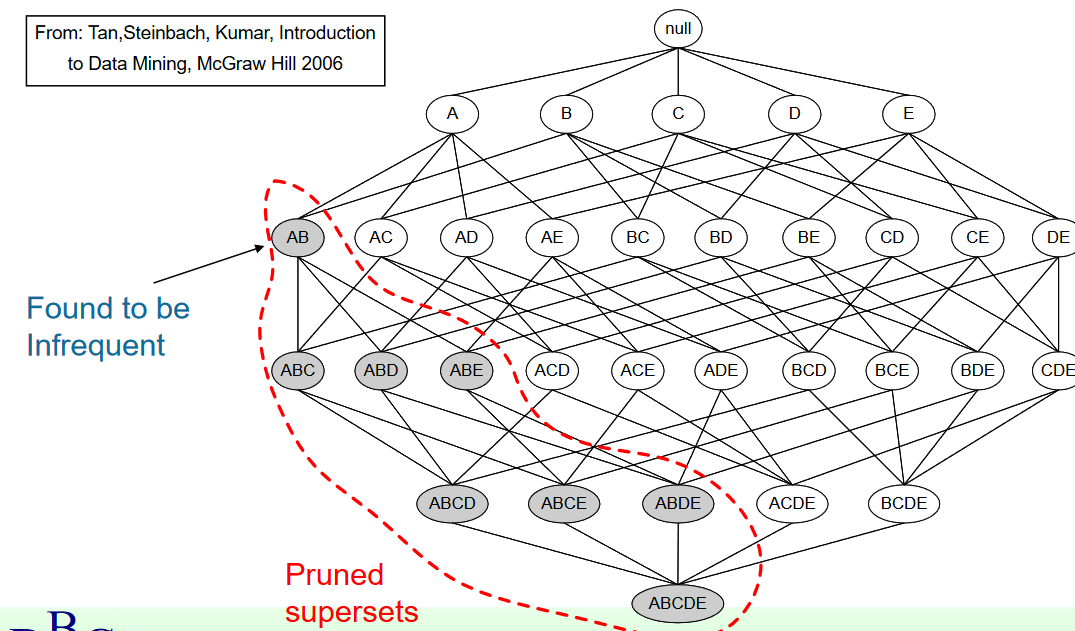
\includegraphics[width=0.8\textwidth]{principio-di-apriori.png}
    \caption{Principio Di Apriori}
    \label{fig:principio-di-apriori}
\end{figure}
L'\textbf{algoritmo di Apriori} si basa sulla suddivisione degli'itemset in  livelli, in ogni livello si prendono dei candidati, facendo il join tra candidati frequenti (che superano la minconf) di livello k si generano candidati di livello k+1, per itemset che non rispettano il criterio di frequenza veiene fatto il pruning dell'albero delle scelte.

Sui candidati di lunghezza 2 va applicato il pruning (apriori). Alla fine si trover\`a l'insieme delle soluzioni che sar\`a l'unione di tutti gli itemset estratti. Pseudocodice:
\begin{lstlisting}[language=java]
candidateItemset = new List<List<Transaction>, List<Integer>>;
frequentItemset = new List<List<Transaction>>;

frequentItemset[1] = {frequentItems};
for (int k = 1; frequentItemset[k].notEmpty(); k++) {
    condidateItemset[k+1] = frequentItemset[k];

    for (Transaction t : db) {
        if (transaction of candidateItemset[k+1] is contained in t) {
            increase the coutnter of that transaction in candidateItemset[k+1];
        }
    }

    frequentItemset[k+1] = candidateItemset[k+1].filter(t -> t has count greater than minsup);
}

return frequentItemset.union();
\end{lstlisting}

\tolerance=1000
Le limitazioni principali di questo algoritmo sono i costi di scansione del database, infatti dovr\`a essere letto pi\`u volte, inoltre se le transazioni sono molto lunghe l'algoritmo dovr\`a essere ripetuto n+1 volte (n = lunghezza transazoine), per superare questo limite si posso usare degli algoritmi per diminuire i costi legati alla lettura.


\subsubsection{FP-Growth}
Sono state proposte delle varianti dell'algoritmo per ottimizzare i problemi . Negli anni 2000 \`e stato proposto un nuovo algoritmo basato sulla memorizzazione. L'algoritmo \textbf{FP-growth}, instazia in memoria un albero dove si trova la proiezione del database originale che considera gli item che soddisfano la soglia di supporto, una volta creata la struttura di supporto in memoria non si accede pi\`u in memoria secondaria, ottimizzando la lettura degli item. La struttura in memoria prende il nome di \textbf{FP-tree}. L'algoritmo funziona nel seguente modo:
\begin{enumerate}
    \tolerance=1000
    \item le transazioni nel db vengono ordinati in base alla cardinalit\`a;
    \item viene creata una header table con le transazioni in orine descrescente, con supporto maggiore della soglia (minsup);
    \item viene scansionato per l'ultima volta il database per creare l'FP-tree;
    \item per ogni transazione viene preso l'item ed inserito nell'albero, ogni nodo contiene l'item ed il numero di volte che \`e stato trovato per ogni transazione letta;
    \item l'inserimento nell'albero viene fatto a partire dall'ordine degli item nella transazione (simile algi alberi formati a partire da ogni lettera di parole), ogni volta che si passa da un nodo gi\`a inserito il suo contatore aumenta, altrimenti si crea un nodo nuovo con count = 1;
    \item \`e importante collegare la header table ai nodi nell'albero, questo viene fatto attraverso una \textbf{node link chain}: l'header punta ad un nodo con lo stesso item, quando percorrendo l'abero si trova un altro item il nodo precedente avr\`a come nodo successivo il nodo corrente;
\end{enumerate}

Viene poposto anche un algoritmo di visita per estrarre gli itemset:
\begin{enumerate}
    \item viene letta la header table dall'item col supporto pi\`u basso;
    \item viene creato un \textbf{conditional pattern base} (CPB) di un item, una proiezione dell'fp-tree condizionato ad un item;
    \item il CPB viene visitato ricorsivamente per travore i candidati;
    \item ad ogni nodo visitato viene recuperato il path dell'albero fino ad esso, se il supporto del nodo \`e minore del minsup il path viene scartato, e si passa al prossimo nodo della node-link chain;
        \begin{figure}[H]
            \centering
            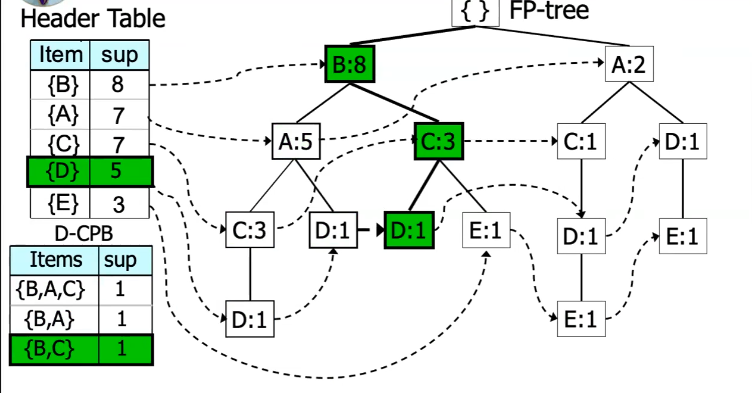
\includegraphics[width=0.8\textwidth]{cpd-di-d.png}
            \caption{Cpd di D al terzo step}
            \label{fig:cpd-di-d}
        \end{figure}
    \item data la cpb va creata una Conditional header table, da questa header table, si crea un'altro fp-tree, questo si applica ricorsivamente, ogni chiamata \`e condizionata (ovvero la cpd sar\`a preceduta dall'itemset del chiamante: $ D -> DC -> \dots$);
    \item quando non si riesce a creare una header table si torna al chiamante e si passa alla entry superiore nella header table del chiamante;
    \item prima di creare la nuova cpb, si prende l'itemset che arriva dal chiamante e se il valore nell'header tabel del item corrente \`e maggiore del minsup allora l'itemset concatenato all'item corrente viene insireti negli itemset frequenti;
        \begin{figure}[H]
            \centering
            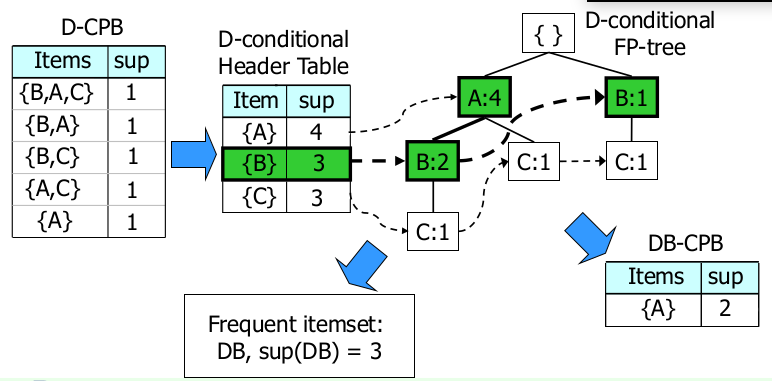
\includegraphics[width=0.8\textwidth]{esempio-aggiunta-itemset-nei-valori-frequenti.png}
            \caption{Esempio Aggiunta Itemset Nei Valori Frequenti}
            \label{fig:esempio-aggiunta-itemset-nei-valori-frequenti}
        \end{figure}
\end{enumerate}
Questo algoritmo funziona molto bene se la memoria non viene saturata (bottleneck).

Un altro problema sono l'alto numbero di itemset che vengono estratti, infatti anche con db molto piccoli si possono trovare un numero molto elevato di iteset frequenti, per questo si opta per i \textbf{itemset massimali frequenti}, IMF per definizioni sono gli itemset che hanno il massimo numbero di figli, e sono unici nel loro sottolivello, oppure esistono i \textbf{closed itemset} che sono gli itemset con nessuno dei suoi immediati superset hanno lo stesso valore.
\[ ItemsetFrequentiMassimali \subset ItesetFrequentiChiusi \subset ItemsetFrequenti \]

\subsection{Effetto delle soglie}
La scelta dei valori di supporto deve essere idoneo, infatti con un valore troppo basso non si identificano delle relazioni che portrebbero risultare interessanti e con valori troppo alti emergono relazioni molto deboli. Anche la confidenza comporta dei problemi, se il valore di cui si calcola la confidenza ha un valore molto ampio, si rischiano di ottenere valori errati, per evitare di incrociare queste informazioni si utilizza la regola del lift.
\begin{definition}{Lift}{lift}
    Dato $ r: A \implies B $, allora la Correlazione o lift \`e:
    \[ C = \frac{P(A,B)}{P(A)P(B)} = \frac{conf(r)}{sup(B)} \]
    \begin{itemize}
        \item $C = 1$: indipendenza statistica;
        \item $C < 1$: correlazione negativa;
        \item $C > 1$: correlazione positiva;
    \end{itemize}
\end{definition}


Un esempio di regola di associazione potrebbe anche essere l'aggregazione di dati, andano ad accoppirare una tassonomia ai valori, possiamo, aggregano gli attribuiti, vedere il loro supporto crescere, rappresetando in modo generalizzato un comportamento, per andare a soddifare un servizio.


\newpage
\section{Classificazione}
Le classificazioni cercano, attraverso dei modelli di assegnare dei tag ai dati, attraverso delle tecniche supervised (vuol dire che abbiamo gi\`a a disposizione un pool di dati da cui possiamo estrapolare le informazioni per assegnare un tipo di tag).

Per applicare la classificazione si ha bisogno di dei dati di training che hanno gia dei tag con il quale si va a generare un modello, per classificare dei nuovi dati si parte dandoli in pasto al modello e partendo dai volori degli attributi si generano delle nuove etichette.

Per poter realizzare un modello di classificazione si ha bisogno di dati di training, usati per generare il modello, e dati di test, usati per validare il modello, ognuno di questi dati ha gi\`a associato ad essi una classe di tag. Una volta che si trova un modello adatto, si pu\`o insireri in un applicazione per predirre i tag.

Gli algoritmi che generano i modelli hanno delle caratteristiche:
\begin{itemize}
    \item accuratezza;
    \item interpretabilit\`a;
    \item incrementalit\`a: il modello pu\`o essere aggiornato all'arrivo di nuovi dati;
    \item efficenza;
    \item scalabilit\`a: performance dell'algoritmo rispetto al numero di dati;
    \item robustezza: capcit\`a dell'algoritmo di operare in presenza di dati rumorosi o mancanti;
\end{itemize}

\subsection{Alberi di Decisione}
Attraverso un albero di decisione, dati i dati di input \`e possibile inferire la classe di etichetta.
\begin{figure}[H]
    \centering
    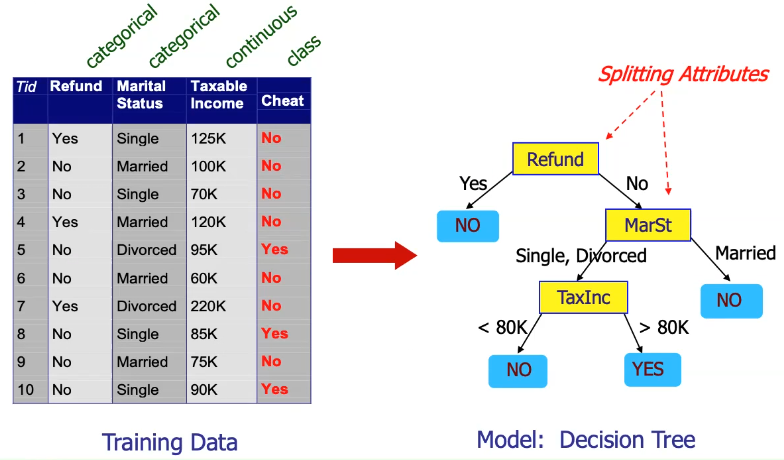
\includegraphics[width=0.8\textwidth]{albero-di-descisione.png}
    \caption{Albero Di Descisione}
    \label{fig:albero-di-descisione}
\end{figure}
In un albero di decisione le folgie corrispondo all'etichetta di classe che sar\`a assegnata all'item in esame. Questo modello dipendo molto dai dati, infatti se gli attributi cambiano anche il modello va modificato opportunamente, questo \`e dovuto al fatto che gli alberi di decsione non sono incrementali. Per generare gli alberi di decisione esistono vari algoritmi, uno di questi \`e l'\textbf{algoritmo di Hunt}, l'algoritmo parte dal leggere il database, il primo passo \`e quello di individuare l'attributo che riesce a dividerere il db in due gruppi pi\`u omogenei possibili rispetto al tag. Successivamente si cerca il prossimo attributo che effettua il prossimo miglior partizionamento, fino al raggiungimento delle condizioni di terminazione. Questo albero non \`e aggiornabile all'arrivo di nuovi dati.

Per effettuare lo split bisogna partire dai tipi di dati con cui si lavora:
\begin{itemize}
    \item attributo categorico: si possono effettuare n-split diversi per ogni valore, se il tag \`e binario allora i valori vengono partizionati in due gruppi;
    \item attributo numerici: si pu\`o usare la discretizzazione, oppure si pu\`o usare una condizione di test;
\end{itemize}

Per stimare la purezza (grado di omogeneit\`a) dei nodi che vengono generati, esistono delle metriche per calcolare l'impurit\`a: gini index, entropia, missclassification index. Il primo caso \`e quello di utilizzo del \textbf{Gini index}, con questo metodo viene misurata l'impuit\`a prima e dopo lo split, il gini index si misura con:
\[ GINI(t) = 1 - \sum_{j}^{} (p(j|t))^{2} \]
$p(j|t) = $ frequenza della classe j al nodo t. Pi\`u il gini index si avvicina allo zero, pi\`u la classe \`e \textbf{pura}, pi\`u il valore si avvicina a $(1 - \frac{1}{\text{numro di classi}} )$ pi\`u il nodo \`e impuro, viene preso l'attributo che genera il gini index col valori pi\`u basso. Nelle implementazioni reali vengono fatti dei test utilizzando metriche diverse con successive validazioni.

Per la creazione di un albero va definito anche un criterio di stop:
\begin{itemize}
    \item minamal gain;
    \item pre-pruning: se un nodo \`e quasi puro rimuovo non scendno pi\`u nell'albero;
    \item post-pruning: generato l'albero completo vado a tagliare i rami dell'albero con delle caratterisiche troppo specifiche;
\end{itemize}



\subsection{Random Forest}
I random forest sono un'estensione degli albri di decisione (pi\`u alberi di descisione), dato un db si creano n sottoinsiemi dei dati originali, su ogni sottoinsieme si crea un albero di decisione, ognuno di questi modelli per decidere l'etichetta, successivamente si seglie l'etichetta finale in base ai voti (possono anche essere pesati).

Si parte con il \textbf{Bootstrap} che va a estrarre gli n sottoinsiemi (con ripescamento) di oggetti randomici, base alla cardinalit\`a, poi si va a creare un albero di decisione applicando una selezione degli attributi (non tutti gli alberi potrebbero utilizzare le stesse feature), ma si scelgono gli attributi che megli modellano i dati che si vogliono analizzare.


\subsection{Rule-based Classification}
Si parte da un database di training. Le classificazione rule-based sono composte da: (conidizione) $ \implies $ y, dove la condizione \`e in inseme di condizioni booleane e y \`e la classe. Un esmpio \`e:
\begin{center}
    (Blood type == warm) \&\& (can fly == yes) $ \implies$ Bird
\end{center}
Dato il db di training si genera il modello, che \`e composto da n regole R.

Ogni regola R che matcha la entry che si sta elaborando, viene associata la classe all'istanza, se esistono delle collisioni, si pu\`o utilizzare la mutua esclusione, e soprattutto (idealmente) le regole devono essere esaustive (non devono esistere casi non gestiti).

Per creare le regole si pu\`o partire da un albero di decisione, in questo modo si risolve la mutua esclusione ma non l'esaustivit\`a. La strategia che solitamente si segue \`e il semplificamento di queste regole, le rogole possono essere semplicate al completamento dell'albero di decisione, oppure si potrebbe semplificare l'albero con del pruning e poi estrarre le regole, oppure estrarre  le regole direttamente dal db. Quando le regole non sono esaustive si una classe di default che solitamente \`e la maggioritaria.

Le caratteristiche di questi modelli sono:
\begin{itemize}
    \item accuratezza maggiore degli alberi di decisione;
    \item interpretabili;
    \item non sono incrementali;
    \item molto efficenti;
    \item sono scalabili sia sul training set che sul numero di attributi;
    \item sono robusti agli outliers;
\end{itemize}


\subsection{Classificazione Associativa}
Si utilizzano le regole di associazione per fare delle previsioni, le regolo di associazione per\`o vanno ristrette, per la classificazione le uniche regole che interessano sono (condizione) $ \implies $ regola di classe (un sottoinsieme delle regole possibili). In questo caso l'estrazione \`e diversa dalle regole di associazione, infatti la classificazoine associativa \`e composta da regole ordinate con degli indice di qualit\`a, l'ordinamento \`e fatto sulle regole di associazione (soglia, confidenza, lift). Anche in questo caso non si vuole fare dell'overfitting sul training set, quindi in fase di creazione si dovr\`a decidere dove fare del pruning.

Le caratteristiche sono:
\begin{itemize}
    \item ha un accuratezza maggiore alla rule-based;
    \item modello iterpretabile;
    \item non incrementale;
    \item efficenza bassa: dato dall'estrazione delle regole di associazione (dato dal minsup);
    \item la scalabilit\`a dipende dai dati: dimensione dell'FP-growhth (ad esempio);
    \item non soffre di missing value e robusti agli outliers;
\end{itemize}


\subsection{K-Neareset Neighbor (KNN)}
\`E un algoritmo di classificazione che non ha un modello, ma si basa sul dataset di training, in questo modo non viene effettuato alcuna fase di training. Quando si vuole classificare un nuovo item, si cercano delle similarit\`a dal dataset di training e poi si assegna la classe. Per decidere quali dati dall'itemset di training sono i pi\`u simili al nuovo item si utilizza un concetto di vicinanza, trovati i sui vicini si assegna la classe, il numero di vicini che vengono scelti \`e dato dal valore K, la scelta di questo valore influisce col rumore che possono causare i vicini. Le misure di distanza dipende dal tipo di dato.

Le caratteristiche sono:
\begin{itemize}
    \item l'accuratezza \`e simile ai precedenti;
    \item il modello non \`e interpretabile;
    \item il training set pu\`o essere incrementale;
    \item tempi di classificazione lunghi;
    \item la scalabilit\`a \`e determinata dalla cardinalit\`a dell'training set;
\end{itemize}


\subsection{Bayesian Classification}
\begin{theorem}{Teorema di Bayes}{teorema-di-bayes}
    \[ P(C,X) = P(X) \cdot P(C|X) \]
\end{theorem}
La classificazione bayesiana si basu sul teorema di bayes, questo tipo di classificazione presuppune un indipendenza statistica dei dati tra di loro, che solitamente \`e l'ipotesi sbagliata. Quando si vuole classificare una nuova tupla X rispetto ad un classe C si calcola $P(X|C)P(C)$ per ogni classe, il valore pi\`u alto trovato corrisponder\`a alla classe di apparteneza delle tupla. Per calcolare $P(X|C)P(C)$ si calcola:
\[ P(C) \prod_{i=1}^{N} P(x_i|C)  \]
dove $x_i$ \`e un attributo della tupla X (\`e per questo motivo che si richiede l'indipendenza statistica, altrimenti quella moltiplicazione non sarebbe possibile).


\subsection{Support Vector Machines}
\`E una tecnica non interpretabile che va identificare un iperpiano che va a separare le classi di interesse. Questo iperpiano deve massimizzare il suo margine (distanza tra l'iperpiano i punti pi\`u vicini delle classi). \`E possibile definire anche delle curve non-lineari modificando il kernel dello spazio vettoriale.

Le caratteristiche sono:
\begin{itemize}
    \item performance tra le migliori;
    \item non interpretabile;
    \item non incrementale;
    \item molto efficente con il giusto tuning;
    \item scalabilit\`a media;
    \item robusti ad outlier e rumori;
\end{itemize}


\subsection{Artificial Neural Network}
L'algoritmo utilizza delle unit\`a di computazioni detti \textbf{neuroni}, questi neuroni sono collegati tra di loro attraverso \textbf{sinapsi}. Esistono vari modelli di rete neurale:
\begin{itemize}
    \item Feed Forward NN: la pi\`u basilare;
    \item Convolutional NN, prima viene modellato il dato utilizzando dei filtri, che poi viene dato ad un FFNN per la computazione finale;
    \item Rcurrent NN, 
    \item auto-encoder: vengono fatte delle elaborazione di dato dove viene fatto del denoising;
\end{itemize}

FFNN si ha un livello di input ed un livello di output ovvero l'etichetta di classe che deve essere predetta, questo modello \`e fully connected, ogni nodo genera un output che va in input ad ongi nodo del livella successivo, questo connessioni sono pesate. Ogni nodo \`e composto da: la somma di tutti gli output pesati, poi questo valore moltiplicato per un coefficiente e poi dato in pasto ad un funzione di attivazione che genera l'output. Le funzioni di attivazione decide come elaborare i valori, le pi\`u utilizzate sono la sigmoide e la tangente iperbolica. Altre funzioni sono il binary step o la rampa. La funzione utilizzata per l'output finale \`e la sofmax. 

Costruire un algoritmo di rete neurale viene fatto con un approccio iterativo:
\begin{enumerate}
    \item ai vettori peso vengono assegnati dei valori casuali;
    \item l'istanza processata veiene processata da tutti i layer della rete, l'output viene confrontato con il vero valore dell'etichetta;
    \item ad ogni iterazione viene fatta una backpropagation per aggiustare i valori dei pesi e dei nodi;
    \item l'iterazione finisce quando si raggiunge una certa percentuale di guess corretti o quando si finisce il dataset di training;
\end{enumerate}

Le caratteristiche sono:
\begin{itemize}
    \item performance migliori;
    \item non interpretabile;
    \item non incrementale;
    \item il training \`e molto lento ma la classificazione \`e molto veloce;
    \item riechede grandi moli di dati ma il training diventa pi\`u lento;
    \item robusti in presenza di dati rumorosi ed outliers, questo \`e ottenuto con un grande pool di dati di test;
\end{itemize}

Un'architettura utilizzata sono le \textbf{Convolutional NN}, la parte di computazione convoluzionale vanno ad effettuare delle feature selection sui dati in input, questi dati vengono poi mandati in input in una rete FFNN. Per estrarre le feature un layer convoluzione fa operazione:
\begin{enumerate}
    \item convoluzione;
    \item funzione di attivazione;
    \item pooling;
\end{enumerate}
I dati sono rappresentati in tensori (matrice multidimensionale), ogni matrice di input \`e un tensore, l'output \`e anch'esso generato in un matrice tensoriale. La convoluzione viene effettuando applicando una finestra di filtro, che viene fatta scivolare su tutto il tensore, solitamnte viene aggiunto un padding ai bordi, ogni eleborzione viene effettuata considerando il vicinato di un punto che genera un singlo punto in output. Dopo la convoluzione viene applicata la funzione di attivazione, solitamnte nelle CNN viene utilizzata la ReLU (rampa). La fase di pooling \`e una fase di downsampling, viene fatto applicando dei filtri al tensore in output, il risultato finale \`e un assegnazione di tag ai vari oggetti presenti nel dato.

Un'altra architettura \`e quello basato sulle \textbf{Recurrent NN} applicate sui tipi di dato con un concetto di tempo, queste architettura hanno un concetto di memoria, infatti all'n-esima elaborazione prendono in considerazione l'elaborazione n-1.

\textbf{Support Vector Machines}



\subsection{Model evuation}
Nella letteratura esitono delle diverse tecniche per decidere quali dati faranno parte della fase di training di un per la creazione di un modello e quali per la validazione del suddetto. Supponiamo di avera un db con 100 oggetti, si vuole utilizzare una parte di questi oggetti per il training associandogli le caratteristiche dell'input e dell'output, si utilizzano gli oggetti rimanenti per validare il modelo creato, verificando il corretto assegnamento delle etichette. 

La prima operazione da effettuare \`e quella di misurare la distribuzione dei tag nei diversi oggetti, calcolare i costi di missclassification e misurare la cardinalit\`a del training set.

Una tecnica di partizione dei dati \`e l'\textbf{hold out}, dove si definiscono delle percentuali fisse tra training e test, generalmente l'80\% dei dati vengono usati per il training ed il 20\% per la validazione. Queste percentuali vanno mantenute per tutte le classi presenti, serve dunque un sampling di tipo stratificato attraverso tutte le classi, questo vuol dire che la percentuale con cui appaiono le diverse classi deve essere mantenuta nei partizionamenti. Questa tecnica \`e utilizzata con db di grosse dimensioni.

La tecnica della \textbf{cross validation} presenta nativamente la ripetizione della fase di training. I dati vengono divisi in k \textbf{fold}, su k-1 fold viene fatto il training mentre sul rimanente viene fatta la validation, questo viene ripetuto per ogni fold. Quando un db \`e piccolo (e.g. nei casi medici), si prendono il numero di fold uguali al numero di entry nel database, quindi prendendo un singolo oggetto viene fatto il tranining su tutti gli altri, questa tecnica viene detta \textbf{leave-one-out}.

Per poter stimare correttamnte un modello deve essere validato in base ai parametri di input (analisi delle sensitivit\`a), si devono selezionare i parametri di input del modello e fare delle validazioni, il motivo per il quale il dataset iniziale viene diviso in tre parti:
\begin{itemize}
    \item parte di training 60\%;
    \item parte di validation (fatto sulla sensitivit\`a dei parametri) 20\%;
    \item parte di test 20\%;
\end{itemize}
L'hold-out viene utitlizzato per dividere il db in training-validation e test, mentre il cross validation divide il db in training e validation.

Esistono delle metriche per poter stimare in modo oggettivo le predizione fatte dal modello, per far questo viene utilizzata la \textbf{matrice di confusione}.
La metrica  dell'accuratezza non \`e sempre affidabile, consideriamo un esempio: 
\begin{table}[H]
    \centering
    \begin{tabular}{|c|c|}
        \hline
        classe & record \\
        \hline
        0 & 9900 \\
        1 & 100 \\
        \hline
    \end{tabular}
\end{table}
assegnando un classificatore di default che assegna sempre la classe 0 la sua accuratezza sar\`a del 99\%, mentre la classe 1 non sar\`a mai predetta, questo \`e un esempio di caso in cui le classi sono sbilanciate, il nostro interesse in questi casi \`e predirre con precisione la classe minoritaria, come nella vita reale solo l'1\% della popolazione contrae una malattia, ma quell'1\% deve esere predetto con la maggiore precisione. Generalmente si danno delle metriche di valore per gli attributi di interesse, queste metriche calcolate pre una classe di interesse vengono dette, \textbf{recall} (numero di oggetti correttamente assegnati alla classe / numbero di oggetti che appartengono alla classe) e \textbf{precision} (numero di oggetti correttamente assegnati alla classe / numbero di oggetti assegnati alla classe). Queste metriche vanno massimizzate attraverso l'\textbf{F-measure} $= \frac{2rp}{r + p} $.

\subsection{Curva ROC}
ROC sta per (Receiver Operating Characteristics), questa curva caratterizza il trade-off tra numero positive di hits e falsi positivi. La curva ROC viene plottata su due assi:
\begin{itemize}
    \item \textbf{TPR}: true positive rate (y);
    \item \textbf{FPR}: false positive rate (x);
\end{itemize}
\begin{figure}[H]
    \centering
    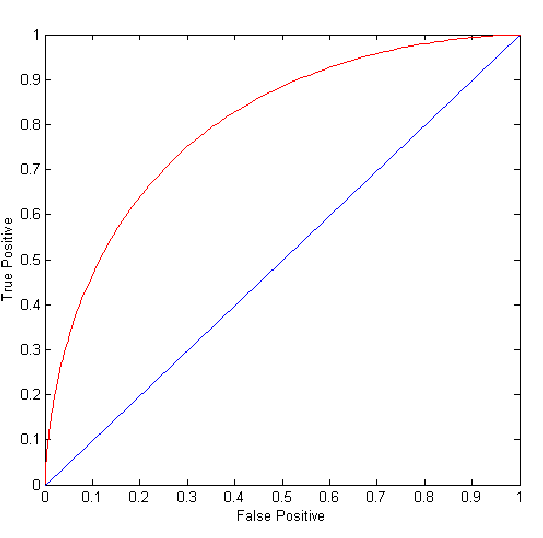
\includegraphics[width=0.8\textwidth]{roc.png}
    \caption{Roc}
    \label{fig:roc}
\end{figure}
Generalmente un curva \`e buona se si trova al di sopra della diagonale.



\newpage
\section{Trigger}
Consideriamo un esmpio di tema di esame.

a:
\begin{lstlisting}[language=sql]
misure: sum(incasso), sum(#consulenze)
tabelle: INCASSO, TEMPO, SERVIZION, SEDE-CONSULENTI
gb: semestre, tipologia-servizio
selezione: regione = 'Lombardia'
\end{lstlisting}

b:
\begin{lstlisting}[language=sql]
misure: sum(incasso), sum(#consulenza)
tabella: INCASSO, SEDE-CONSULENTI, SERVIZIO, TEMPO, AZIENDA
gb: regione, servizio, anno
selezione: Nazionalita = 'Italia' or
    Nazionalita = 'Germania'
\end{lstlisting}

c:
\begin{lstlisting}[language=sql]
misure: sum(incasso), sum(#consulenze)
tabelle: INCASSO, SEDE-CONSULENTI, SERVIZIO, TEMPO
gb: tipologia-servizio, regione, semestre
selezione: anno >= 2017 and anno <= 2019
\end{lstlisting}

Date le query precedenti si crei una vista materializzata:
\begin{lstlisting}[language=sql]
-- Query blocco A
select servizio,
    tipologia-servizio,
    semestre,
    anno,
    regione,
    nazionalita,
    sum(incasso),
    sum(#consulenze)
from incasso i, tempo t, azienda a, servizio s, sede-consulenze sc
where condizioni di join
group by servizio,
    tipologia-servizio,
    semestre,
    anno,
    regione,
    nazinalita
\end{lstlisting}

L'identificare minimale sar\`a: (servizio, semestre, regione, nazionalita)

Punto 2:
...

Punto 3:
\begin{lstlisting}[language=sql]
insert into viewIncassi(servizio,
    tipologia-servizio,
    nazionalista,
    semestre,
    anno,
    regione,
    incassotot,
    numconsulenzetot)
(blocco A)
\end{lstlisting}

Punto 4:
\begin{lstlisting}[language=sql]
create trigger refreshViewIncassi
after insert on incasso
for each row
declare
    varServizio varchar(20);
    varTipologiaServizio varchar(20);
    varSemestre varchar(20);
    varAnno varchar(20);
    varNazionalita varchar(20);
    varRegione varchar(20);
    n int;
begin
-- leggere le tabelle dimensionale x recuperare
-- i valori dell'identificatore della vista materializzata:
-- servizio, nazionalita, semestre, regione
select servizio, tipologia-servizio into varServizio,
    varTipologiaServizio
from servizio
where idServizio = :NEW.idServizio;

select semestre, anno
from tempo
where idTempo = :NEW.idTempo;

select nazionalita into varNazionalita
from azienda
where idCategoriaAzienda = :NEW.idCategoriaAzienda

select regione into varRegione 
from sede-consulenti
where idSede = :NEW.idSede;

-- verifico se esiste una tupla in viewIncassi con
-- associati i valori estratti

select count(*) into n
from viewIncassi
where nazionalita = varNazionalita and
    semestre = varServizio and
    servizio = varServizio and
    regione = varRegione;

if (n > 0) then
    update viewIncassi
    set incassoTot = incassoTot + :NEW.incasso
        numConsulenze += :NEW.#consulenze
    where servio = varServizio and
        nazionalita = varNazionalita and
        semestre = varSemestre and
        regiono = varRegione;
else 
    insert into viewIncassi ( ... , )
    values (varServizio,
        varTipoServizio,
        varNazionalita, 
        varSemestre,
        varAnno,
        varRegione, 
        :NEW.incasso,
        :NEW.#consulenze);
end if;
end;
\end{lstlisting}

Punto 5:
\begin{lstlisting}[language=sql]
create trigger updateViewIncassi
after update of tipologiaServizion on servizio
for each row
declare
    typeServizio varchar(20);
begin


end;
\end{lstlisting}

Punto 6:
\begin{lstlisting}[language=sql]
create materialized view log on incasso
with sequence, row id
(...) 
including new values;

create materialized view log on servizio
with sequence, row id
( ... )
including new values;

create materialized view log on tempo
with sequence, row id
(. ...)
including new values;
\end{lstlisting}


\newpage
\section{Lab 03}
1.
\begin{lstlisting}[language=sql]
select mese, tariffa,
    sum(prezzo),
    sum(sum(prezzo)) over () as prezzo_comp,
    sum(sum(prezzo)) over (partition by mese) as prezzo_per_mese,
    sum(sum(prezzo)) over (partition by tipo_tariffa) as prezzo_per_tariffa
from tempo te, fatti f, tariffa t
where te.id_tempo = f.id_tempo and
    f.id_tar = t.id_tar ans
    anno = 2003
group by mese, tipo_tariffa;
\end{lstlisting}


2.
\begin{lstlisting}[language=sql]
select mese
    sum(chiamate) as chiamte_tot,
    sum(sum(prezzo)) as incasso_tot,
    rank() over (
        order by sum(prezzo) desc
    ) as rank_piu_chiamate
from fatti f, tempo t
where f.id_tempo = t.id_tempo
group by mese;
\end{lstlisting}

3.
\begin{lstlisting}[language=sql]
select mese
    sum(chiamate) as chiamte_tot,
    sum(prezzo) as incasso_tot,
    rank() over (
        order by sum(chiamate) desc
    ) as rank_piu_chiamate
from fatti f, tempo t
where f.id_tempo = t.id_tempo and
    anno = 2003
group by mese;
\end{lstlisting}

4.
\begin{lstlisting}[language=sql]
select tipo_tariffa
    sum(prezzo)
from fatti f, tariffa t
where f.id_tar = t.id_tar and
    mese = 'luglio' and
    anno = 2003
group by tipo_tariffa;
\end{lstlisting}

5.
\begin{lstlisting}[language=sql]
select mese
    sum(prezzo) as incaso_tot,
    sum(sum(prezzo)) over (
        order by mese
        rows unbounded preceding
    ) as incasso_da_inizio_anno
from fatti f, tempo t
where f.id_tempo = t.id_tempo
group by mese;
\end{lstlisting}

6.
\begin{lstlisting}[language=sql]
select tipo_tariffa, mese,
    sum(sum(prezzo)) over (partition by mese) as incasso_per_mese,
    sum(sum(prezzo)) over (partition by tipo_tariffa) as incasso_per_tariffa,
    100 * sum(sum(prezzo)) over (partition by mese) /
        sum(sum(prezzo)) over (partition by tariffa)
from fatti f, tempo t
where f.id_tempo = t.id_tempo and
    anno = 2003
group by tipo_tariffa, mese;
\end{lstlisting}

vista:
\begin{lstlisting}[language=sql]
create materialed view view_fatti
biuld immediate
as
select mese,
    tipo_tariffa,
    anno,
    sum(prezzo) as prezzo,
    sum(chiamate) as chiamate
from fatti f, tempo te, tariffa t
where f.id_tempo = te.id_tempo and
    f.id_tar = t.id_tar and
    anno = 2003
gorup by mese,
    tipo_tariffa,
    anno,
    prezzo,
    chiamate;
\end{lstlisting}



\newpage
\section{Clustering}
Il clustering consiste nel raggruppamento di oggetti similiri tra di loro, questa tecnica viene detta di \textbf{unsupervised learnig} perch\`e per effettuare questa suddivisione parte solo da informazioni presenti nei dati. Le tecniche del cluster analysis si pone l'obbiettivo di partizionare il db in sottogruppi, dove gli oggetti in un sotto grupposono vicini tra di loro mentre sono distanti con gli oggetti degli altri sottogruppi. Col termine clustering si definiscono dei cluster, ovvere degli insiemi di dati, il clustering si suddivide in: partizionale (i dati appartengono ad uno ed us solo gruppo), gerarchico (elementi rappresentati da un albero gerarchico, che identifica n partizionamenti detto dendogramma). Gli algoritmi di clustering possono suddivisi per i gruppi di cluster che si vengono a formare, uno di questi \`e il partizionamento esclusivo vs non-escusivo un punto pu\`o appartenere a pi\`u sottogruppi, fuzzy vs non-fuzzy dove un punto \`e associato ad ogni gruppo ma con un peso per ognuno di essi, parziale quando il partizionamento viene assegnato solo ad sottogruppo esculdendo i dati rumorosi, completa quando ad elemento viene associato un tag. I gruppi identificati possono essere caratterizzati da: cardinalit\`a, densit\`a, forma; esistono degli algoritmi in grado di indentificar\`a gruppi a densit\`a omogenea ed eterogenea, per ogni caratteristica esiste un tipo di algoritmo. I gruppi che si ottengono possono essere:
\begin{itemize}
    \item ben separati: distanza massimizzate tra gruppi diversi e minimizzate tra elementi di un gruppo;
    \item center-based: gruppi rappresentati da un punto medio, \textbf{centroide} media dei punti in cluster, \textbf{medoide} media dei punti pi\`u rappresentativi del cluster;
    \item cluster continui;
    \item density-based: i cluster hanno dansit\`a uguale;
    \item cluster concettuali;
\end{itemize}

\subsection{K-means}
Ogni cluster \`e associato con un centroide, l'algoritmo prende in input un parametro K che corrisponde al numero di cluster. L'algoritrmo \`e formato da:
\begin{lstlisting}[language=]
seleziona K centroidi casuali
do
  si formano K cluster a partire dai centroidi assegnando i valori pi\`u vicini
  si ricalcolano i centroidi a partire dai cluster
while (i centroidi non cambiano)
\end{lstlisting}
Questo algoritmo converge abbastanza velocemente infatti ha O(num-punti * K * iterazioni * num-attributi), per questo motivo l'algoritmo viene fatto eseguire molteplici volte per eliminare il problema dell'assegnazione casuale dei centroidi che potrebbe a portare anche a cluster vuoti. Per valutare quanto \`e buono un partizionamaneto si usa l'SSE, Sum of Squerd Error.
\begin{definition}{SSE}{sse}
    \[ SSE = \sum_{i=1}^{K} \sum_{x \in C_i}^{} dist^{2}(m_i, x) \]
\end{definition}
Questa metrica \`e molto buona per calcore devese run dell'algoritmo su stessi K (o anche comparare le prestazioni di diversi algoritmi), se per\`o si decide di aumentare K allora l'SSE \`e sempre confrontabile ma i valori saranno pi\`u piccoli al crescere di K, perch\`e la base dati rimane la stessa, dunque con pi\`u partizionamento i dati sono molto pi\`u coesi tra di loro.

Oltre ad utilizzare l'approccio delle \textbf{run multiple} si possono utilizzare come centroidi utilizzando punti del database stesso usando altre tecniche. Si possono anche utilizzare centroidi maggiori di K e poi al termine delle run scegliere tra questi i centroidi iniziali, si pu\`o anche utilizzare del postprocessing o un bisect K-means.

Esiste il problema dei cluster vuoti quando si fanno delle iterazioni, per evitare che vengano creati cluster vuoti si prende un punto dal cluster conl'SSE pi\`u grande oppure scegliere il punto con l'SSE pi\`u grande, riassegnando il centroide col un cluster vouto al punto estratto si risolve questo problema, se pi\`u cluster sono vuoti si ripente fino ad otterli tutti con almeno un elemento.

Per ridurre il rumore dei dati eliminando gli outliers si possono applicare operazioni di pre-processing. Una volta finito l'algoritmo si possono applicare operazioni di post-processing come: eliminare cluster piccoli, eliminare cluster con SSE molto grande, oppure fare il merge di cluster vicini tra di loro, per le operazioni di post-processing non esistono delle linee guida, ma solitamente dipende dal contesto.


\subsection{Bisecting K-means}
Il bisecting

...




\section{Introduzione ai DBMS}
Il DBMS permette di avere una gestione concorrente delle informazioni, oltre ad avere delle routine che operano sui dati, la sua struttura \`e molto complessa ed \`e strutturata in moduli, l'entry poiont \`e una query.
\begin{figure}[H]
    \centering
    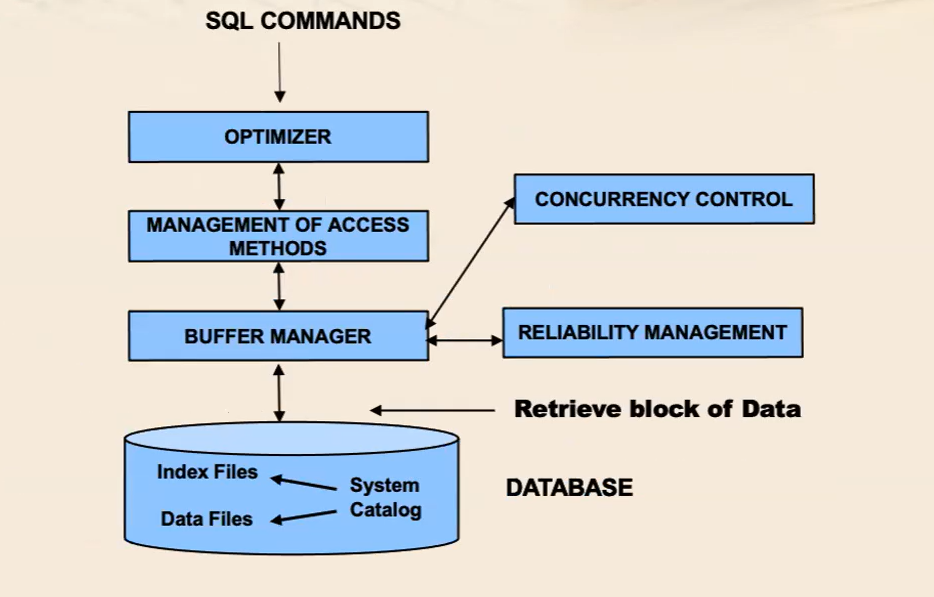
\includegraphics[width=0.8\textwidth]{architettura-dbms.png}
    \caption{Architettura Dbms}
    \label{fig:architettura-dbms}
\end{figure}
Il DBMS \`e composto da:
\begin{itemize}
    \item ottimizzatore: prende delle decisioni in base alla distribuzione dei dati, oltre a fare il parsing della stringa;
    \item access method manager: viene eseguito un metodo specifico per leggere la memoria;
    \item buffer manager: buffer nella moria principale che ottimizza le operazioni di I/O;
    \item concurrency control: gestisce l'accesso concorrente ai dati;
    \item reliability manager: garantisce la correttezza del contenuto dei dati del db, utilizzando dei file di log in cui vengono scritte le operazioni effettuate;
\end{itemize}

Il concetto fondamentale nel constesto dei db sono le \textbf{transazioni}: ovvero di una serie di operazioni che rappresentano una singola unit\`a  di lavoro. Una transazione termina con COMMIT o ROLLBACK. Le transazioni sono caratterizzazate da ACID:
\begin{itemize}
    \item \textbf{atomic}: tutte le operazione dovono andare a buon fine o nessuna, le operazioni che controllono lo stato del sistema sono \textbf{UNDO} o \textbf{REDO};
    \item \textbf{consistency}: non vanno violati i vincoli di consistenza del DBMS, vincoli di chiava, chiave esterna, ...;
    \item \textbf{isolation}: la transazioni operano in modo indipendente tra di loro, i dati intermedi non sono visibili all'esterno;
    \item \textbf{durability}: i dati di una transazione non possono essere persi, questa proprit\`a \`e garantita dal reliability manager;
\end{itemize}


\subsection{Buffer Manager}
Il buffer manager ha accesso ad una parte della memoria principale a cui gli applicativi hanno accesso. Il buffer \`e organizzato in \textbf{parole} o \textbf{pagine} di dati, che \`e l'unit\`a minima trasferibile dalla memoria secondaria, per essere efficace nelle operazioni di IO le pagine devono essere presenti nel buffer per velocizzare le operazioni, per questo motivo si utilizza il principio di localit\`a. Ogni pagina deve avere:
\begin{itemize}
    \item l'ID del file;
    \item l'ID del blocco;
\end{itemize}
Per ogni pagina esistono anche due stati:
\begin{itemize}
    \item \textbf{count}: numero di transazioni che stanno utilizzando la pagina;
    \item \textbf{dirty bit}: settato quando la pagina \`e stata modificata e non \`e stata ancora caricata nella memoria secondaria;
\end{itemize}
\begin{figure}[H]
    \centering
    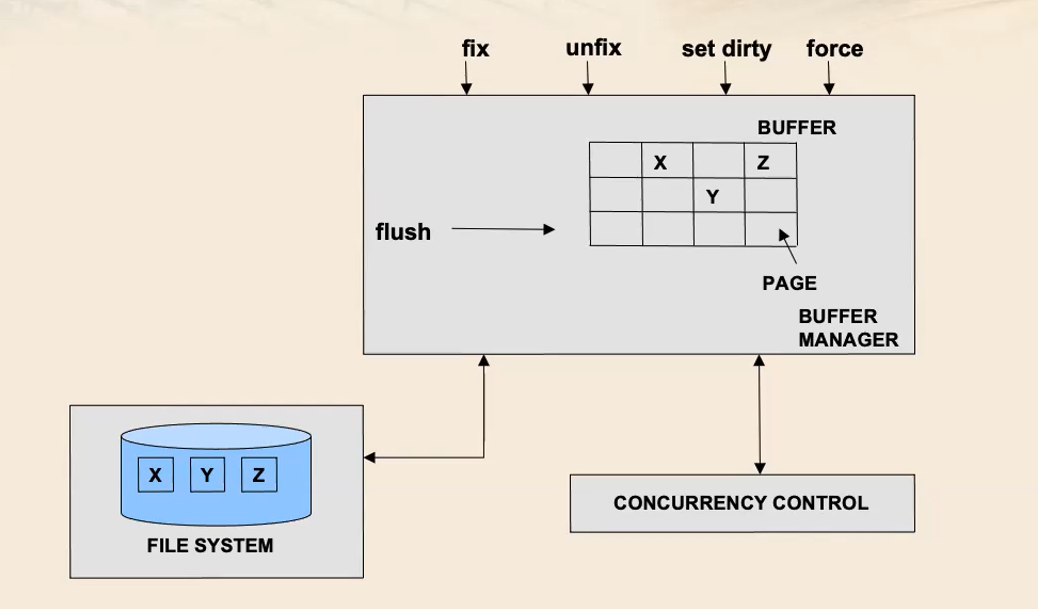
\includegraphics[width=0.8\textwidth]{buffer-manager.png}
    \caption{Buffer Manager}
    \label{fig:buffer-manager}
\end{figure}

Il buffer manager ha a disposizione una parte della memoria principale in cui salva delle pagine di dati dal DB quando viene fatta una query. Eisitono delle primitive per poter accedere a questa memoria:
\begin{itemize}
    \item \textbf{fix}: richiesta dalla transazione, se la pagina \`e disponibile allora viene passata, altrimeti si fanno delle operazioni di IO per recuperare la pagina, se il buffer \`e pieno un'altra pagina deve essere rimpiazzata, solitamente sar\`a un pagina con il \textbf{count}=0, questa pagina viene detta \textbf{vittima} e verr\`a rimpiazzata con qualla richiesta dalla transazione; se durante la transazione una pagina ha il \textbf{dirty biy} = 1 allora deve essere fatta un operazione di IO per sincronizzare la pagina. Prima che la lettura inizii il count viene incrementato di 1;
    \item \textbf{unfix}: viene richiesta dalla transazione quando la pagina non deve essere utilizzata;
    \item \textbf{set dirty}: setta il valore dirty ad una pagina quando viene fatta un'operazione di scrittura;
    \item \textbf{force}: richiede un trasferimento sincrono della pagina al disco, quindi si scrive la pagina, non \`e detto che la pagina venga rimossa;
    \item \textbf{flush}: richiede un trasferimento asincrono della pagina al disco;
    \item \textbf{steal}: quando si utilizza steal il buffer manager pu\`o selezionare una pagina locked con un count=0, detta pagina \textbf{vittima}, e la rimuove dal buffer, se non-steal \`e settato non si pu\`o selezionare una pagina su cui sta avvenendo una transazione;
    \item \textbf{force}: tutte la pagine di una transazione sono scritte in modo sincrono sul disco;
    \item \textbf{no-force}: utilizza flush per scrivere le pagine in modo asincrono sul disco;
\end{itemize}
Inoltre il buffer manager mette a disposizione:
\begin{itemize}
    \item squential read;
    \item write and sequential write;
    \item directory;
\end{itemize}










\subsection{Accesso alla Memoria}
L'access methods manager riceve dall'ottimizzatore il piano di esecuzione e decide quale metodo di accesso utilizzare per leggere o scirvere i dati, vengono poi selezionati i blocchi dei file da prendere dalla memoria principale, questi dati sono richiesti al buffer manager.

Le strutture fisiche che si possono utilizzare sono dipendenti dal tipo di operazione che si effetuano su di loro (select, update, delete, ...), queste strutture sono dette di tipo \textbf{accessorio}, in particolare gli \textbf{indici}, che sono sturtture definite all'interno del db per velocizzare le operazioni di IO. I dati fisici posso essere salvati in strutture sequenziali o strutture di heap, mentre gli indici utilizzano strutture ad albero, bitmap, unclustered hash.

Nelle strutture squenziali le tuple sono storicizzate nella pagina seguendo l'ordine di inserimento, il vantaggio \`e che lo spazio occupato \`e massimo all'interno della pagina e che l'inserimeto \`e molto veloce, quando si fanno delle operazione di delete si vengono a creare dei buchi, mentre con l'update si rischia di scrivere pi\`u dati di quelli che avevo prima.

Gli \textbf{heap file} utilizzano delle strutture secondarie per avvalersi di ricerca veloce, tutti i tipi di operazione sono identiche a quelle delle strutture sequenziali.

Le \textbf{ordered sequential structures} sono delle strutture sequenziali ordinate in base ad una chiave di ordinamento. I dati oridinati servono per velocizzare le operazioni per quelle interrogazioni che usano la stessa chiave di ordinamento. Come contro le operazioni di delete e inserimento sono molto onerose. Viene lasciato dello spazio in pi\`u per eventuali operazioni di update, oppure viene implementato un file di \textbf{overflow}, dove vengono salvati la parte di dati che dopo un'update o insert non entra nella pagina.

Nelle \textbf{strutture ad albero} nei nodi si trovano solo le chiavi per effettuare la ricerca, negli indici unclustered le foglie si trovano parte dei valori della tuple e il puntatore alla tupla originale, mentre in una struttura clustered le foglie corrispondono ai puntatori della tupla, inoltre da una folgia si pu\`o passare all'altra essendo tutte ordinate in modo seequenziale (come nei \textbf{B+-Tree}.
\begin{figure}[H]
    \centering
    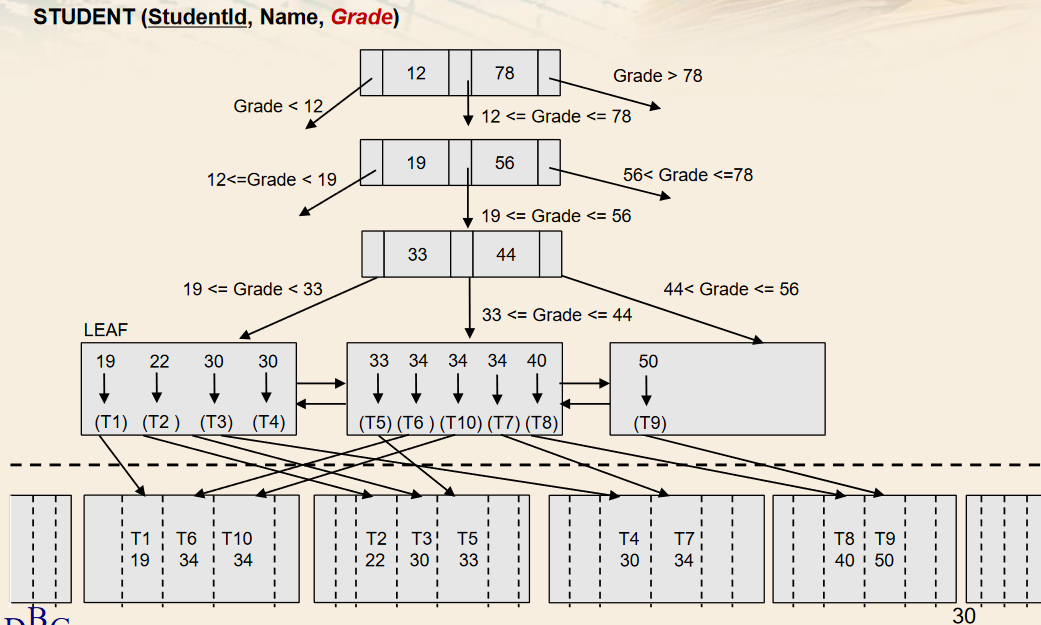
\includegraphics[width=0.8\textwidth]{unclustered-b-tree.png}
    \caption{Unclustered B+-Tree Index}
    \label{fig:unclustered-b-tree}
\end{figure}
\begin{figure}[H]
    \centering
    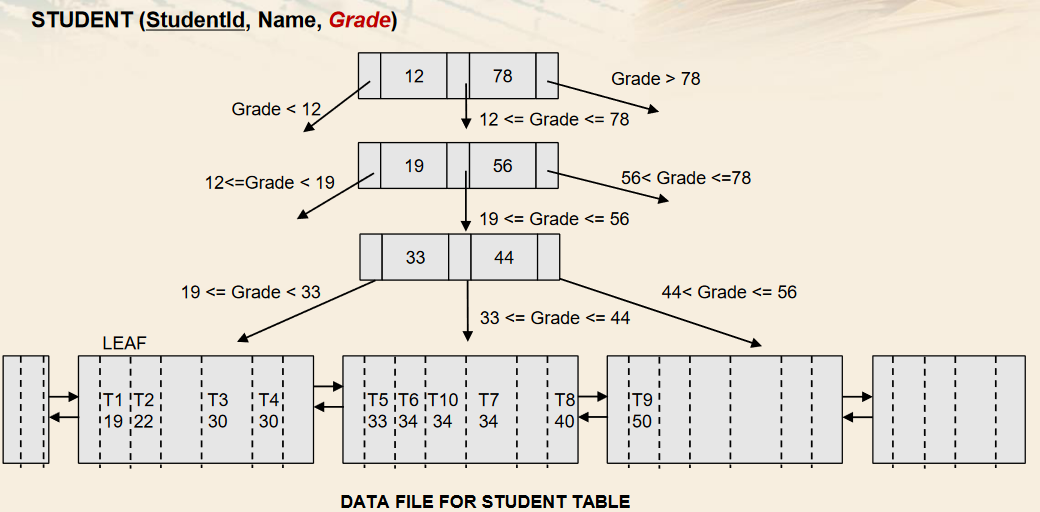
\includegraphics[width=0.8\textwidth]{clustered-b-tree.png}
    \caption{Clustered B+-Tree Index}
    \label{fig:clustered-b-tree}
\end{figure}
Su una tabella pu\`o essere creato un unico indice di tipo clustered, mentre possono essere create pi\`u strutture unclustered.


Un altre struttura utilizzabile \`e la \textbf{struttura di hash}, utilizza una funzione di hash per assegnare ad ogni tupla secondo una chiave, un blocco tra quelli predefiniti della struttura, anche le strutture di hash possono essere clustered o unclustered.


I \textbf{bitmap index} sono delle strutture unclustered, che si portano bene a rappresentare gli attributi categorici.



\subsection{Progettazione Fisica}
Per fare una buona progettazione fisica servono
\begin{itemize}
    \item il progetto logico;
    \item il carico di lavoro in termine di query e frequenza di esecuzione;
    \item engine del database;
\end{itemize}
Nella progettazione fisica dato il carico delle query vengono definiti uno o pi\`u indici e le strutture dati.
\begin{theorem}{Euristiche sulla progettazione fisica}{euristiche-sulla-progettazione-fisica}
\begin{itemize}
    \item mai indicizzare una tabella piccola;
    \item mai indicizzare un attributo con bassa cardinalit\`a;
    \item analizzare i predicati nelle clausole \texttt{where};
    \item quando si creano degli indici composti si deve considerare il costo del mantenimento;
    \item per migliorare le operazioni di \texttt{join} si usano il \textbf{nested loop} (quando si joina un tabella piccola con una grande), ed il \textbf{merge scan} (vengono ordinate le tabelle prima di fare il join);
    \item per le group by si usa un ordinamento una struttura di hash, l'ottimizzatore spesso anticipa le operazioni di group by (\textbf{group by push down}) diminuendo di molto la cardinalit\`a dei dati da analizzare;
\end{itemize}
\end{theorem}
Nelle condizioni di join vengon definite due tabelle:
\begin{itemize}
    \item \textbf{outer}: tabella letta in modo sequenziale;
    \item \textbf{inner}: tabella letta n volte, tante quante le righe della tabella outer;
\end{itemize}
Le alternative per il join sono:
\begin{itemize}
    \item hash join;
    \item nested loop: se la tebella \`e piccola comunque non si indicizza;
\end{itemize}
Se si decide di creare un indice composto \`e meglio che l'indice sia \textbf{coprente}, ovvero che leggendo l'indice si riesce a rispondere alla query senza leggere la tabella, altrimenti diventa troppo oneroso manterlo, diventa pi\`u efficace un indice su un solo attributo.



\subsection{Ottimizzatore delle query}
L'ottimizzatore delle query garantisce efficenza ed indipendenza dai dati. L'ottimizzatore genera un piando di esecuzione, basandosi su delle statistiche, come sulla distrubuzione dei valori e di come quei valori sono distribuiti nei vari blocchi fisici, le soluzioni sono dinamiche, infatti al cambiamento dei dati pu\`o cambiare anche il piano di esecuzione.
\begin{figure}[H]
    \centering
    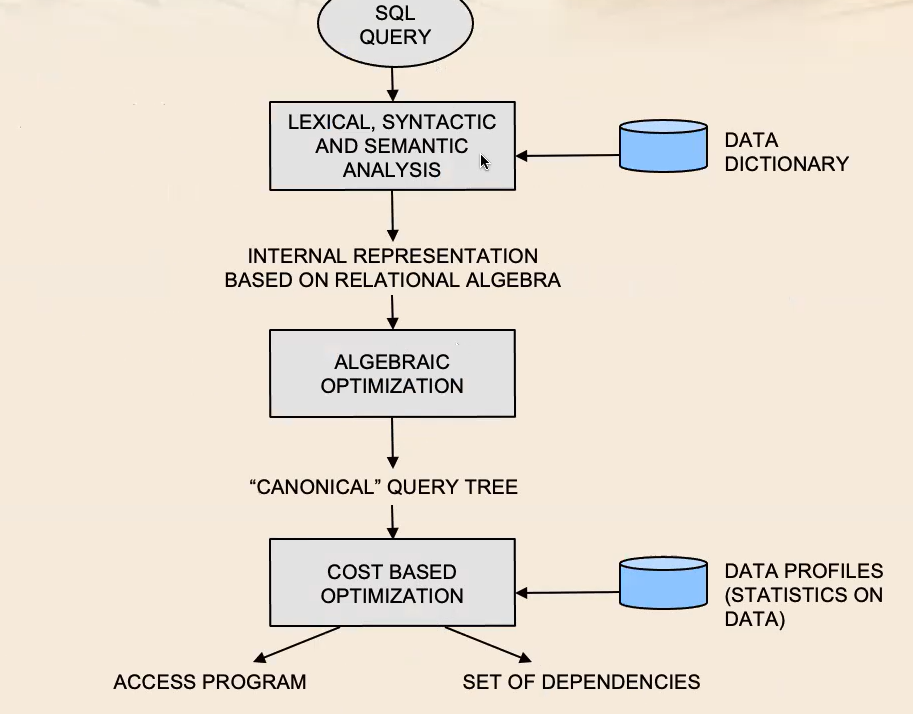
\includegraphics[width=0.8\textwidth]{schema-ottimizzatore.png}
    \caption{Schema Ottimizzatore}
    \label{fig:schema-ottimizzatore}
\end{figure}
L'ottimizzatore fa un controllo su:
\begin{itemize}
    \item errori lessicali: misspelled keywords;
    \item errori sintattici: errori nella grammatica dell'sql;
    \item errori semantici: viene utilizzato il data dictionary per contorllare se un oggetto esiste;
\end{itemize}
Effettuati i controlli genera un rappresentazione interna in algebra relazionale. Il passaggio successivo \`e l'ottimizzazione algebrica, creando un albero di esecuzione. Un volta creato l'albero viene fatta un'ottimizzazione basata sui costi di accesso, quindi ad ogni parte dell'albero vengono assegnati dei punti di accesso. L'ottimizzatore pu\`o essere utilizzato in due modalit\`a:
\begin{itemize}
    \item \textbf{compile and go}: una query non viene salvata, ma viene ricompilata ogni volta, utile quando i dati variano abbastanza frequentemente nel tempo;
    \item \textbf{compile and store}: la query viene compilata e salavta per riutilizzi successivi;
\end{itemize}


\subsubsection{Ottimizzazione algebrica}
Si basa su regole di ottimizzazione dell'algebra relazionale e sulle staistiche dei dati. Esistono delle trasformazioni che si possono applicare alle equazioni dell'algebra relazionale:
\begin{itemize}
    \item 
    \item 
\end{itemize}

\subsubsection{Ottimizzazione basata sui costi}
Per fare una ottimizzazione basata sui costi \`e necessario un modulo Nel \textbf{data profile} sono presenti:
\begin{itemize}
    \item cardinalit\`a delle tuple;
    \item numero di byte delle tuple;
    \item numero di byte degli attributi di una tupla;
    \item numero di valori distinti;
    \item valori minimi e massimi di un attributo;
\end{itemize}
Se la query \`e compile and go in output si avr\`a solamente le modalit\`a di accesso, altrimenti se le query \`e complilata insieme al piano di esecuzione vengono passete l'insieme di dipendenze, grazie a questo insieme si dicideranno se la query dovr\`a essere modificata per soddisfare i cambiamenti che avvengono al db col passare del tempo.




\subsection{Operatori di accesso}
La reppresentazione interna dell'ottimizzatore \`e una query tree. Quando si effettua la lettura delle tabelle si valutano i predicati di selezione, il predicato viene applicato in fase di lettura, anche attraverso utilizzo di index. Anche il join \`e un operazione molto complessa, nei dbms esistono diversi tipi di join:
\begin{itemize}
    \item \textbf{nested loop}: ci sono due tabelle sbilanciata, una grande ed una piccola, per ogni tuple della outer table (grande) viene effettuata una scansione delle inner table (piccola), un eventuale indice creato sulla inner table potrebbe velocizzare l'operazione di join;
    \item \textbf{merge scan join}: tiene conto dell'ordinamente delle tabelle rispetto all'attributo di join, se le tabelle non sono ordinate allora viene fatto un sort;
    \item \textbf{hash join}: viene applicata una funzione di hash rispetto agli attributi della condizione di join, all'interno delle tabella vengono creati dei bucket, all'interno i dati vengono ordinati e poi viene fatto il join tra i bucket;
    \item \textbf{bitmapped join}: \`e una specie di index definito sui dati (infatti questo join \`e dipendente dai dati, non come le altre tipologie di join), viene create una bitmap, ogni riga con la rowid della tabella originale e gli attributi che soddisfano la query hanno un 1, mentre gli attributi che non la soddisfano hanno uno zero;
\end{itemize}
L'operazion di group by possono essere velocizzata con:
\begin{itemize}
    \item \textbf{sort based} prima con un ordinamento e poi con una selezione;
    \item \textbf{hash based}: la tabella viene bucketizzata;
    \item \textbf{materialized views}: con query rewriting;
\end{itemize}



\subsection{Piani di esecuzione}
A differenza dell'obbittivo della query esistono diversi tipi di esecuzione, se i dati servono il prima possibile si trovano dei metodi da inziare a mandarli appena sono disponibili, mentre nella applicazione di tipo batch ci\`o che conta \`e solo il tempo complessivo;
\begin{lstlisting}[language=sql]
select snam, s.id
from exam e, student s
where s.sid = e.sid and score >= 27
order by sname;
\end{lstlisting}
Esempio di piano di esecuzione.
\begin{figure}[H]
    \centering
    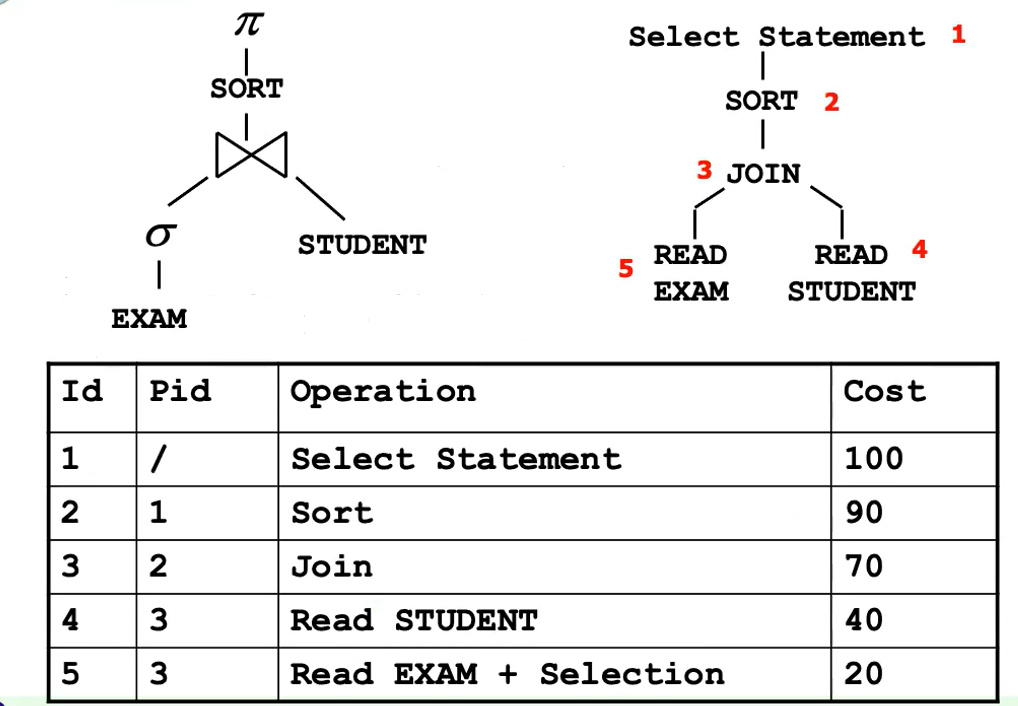
\includegraphics[width=0.8\textwidth]{esecuzione1.png}
    \caption{Esecuzione1}
    \label{fig:esecuzione1}
\end{figure}
Gli accessi alle tabelle possono essere diretti o attraverso gli index, se gli index sono ricoprenti non c'\`e bisogno di accedere alla tabella.
\begin{itemize}
    \item \textbf{full table scan}: lettura sequenziale della tabella, processando in contemporanea i predicati della where, in oracle esiste una funzione che permette di leggere pi\`u pagine di una tabella per velocizzare le operazioni di IO, infatti quando il dbms legge un qualcosa viene sempre letta l'unit\`a minima (pagina), per sapre la distribuzione dei dati nella pagine esiste l'\textbf{index clustering factor}, ovvero quanto i dati sono vicini nei blocchi, se l'ICF \`e alto allora potrebbe essere ottimale leggere la tabella con un index, se \`e basso allora conviene leggere al tabella;
    \item ...
\end{itemize}
Esistono anche dei metodi di lettura relative agli index:
\begin{itemize}
    \item \textbf{index unique scans}: viene utilizzato quando l'attributo su cui \`e stato creato l'indice \`e \texttt{UNIQUE}, l'indice per ogni valore della chiave ritorna un solo valore;
    \item \textbf{index range scan}: dalla lettura dell'indice si possono ottenere pi\`u rowid, ordinati in modo ascendente;
    \item \textbf{index full scan}: si legge tutto l'indece, questo si fa quando non si ha un predicato ben preciso, il vantaggio \`e che i dati vengono restituiti ordinati rispetto alla chiave dell'indice;
    \item \textbf{fast full index scan}: viene utilizzato quando l'indice \`e coprente (non si accede alla tabella), ma si perde l'ordinamento della chiave dell'indice;
    \item \textbf{rowid}: riceve in input il rowid presente nell'index corrispondente a quella della riga della tabella a cui sta puntando;
\end{itemize}
Il data dictionary sono delle tabelle con statistiche sui dati presenti nelle tabelle del db, oracle per immagazzinare informazioni sulle colonne utilizza gli \textbf{istogrammi}. Gli istogrammi sono:
\begin{itemize}
    \item \textbf{height-balanced}: si ha la distribuzione dei valori assunti dall'attributo, i valori vengono distribuiti in intervalli di uguale lunghezza. L'istogramma divide gli intervalli in bucket, il loro valore corrisponde al valore pi\`u grande all'interno del bucket;
        \begin{figure}[H]
            \centering
            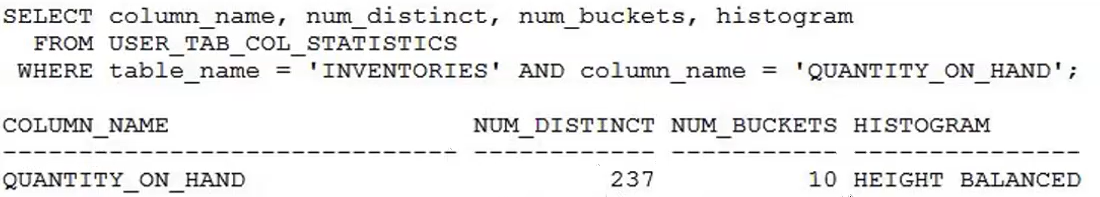
\includegraphics[width=0.8\textwidth]{tipo-di-istogramma.png}
            \caption{Tipo Di Istogramma}
            \label{fig:tipo-di-istogramma}
        \end{figure}
    \item \textbf{frequency}: viene indicata le frequenza dei diversi valori, sempre tra i diversi bucket;
\end{itemize}
Un'altra opzione pu\`o essere la specifica per il miglior \textbf{throughput} (applicazioni batch) ed il miglior \textbf{response time} (applicazioni real time).




\subsection{Regole per valutazione di ottimizzazione}

\begin{theorem}{Regole ottimizzazione}{regole-ottimizzazione}
    REGOLE EURISTICHE:
    \begin{itemize}
        \item tabella piccola:
            \begin{itemize}
                \item piccola se le tuple sono $ \leqslant10^{3}$, no indice;
                \item medio/grande $ > 10^{3} ~ 10^{4}$, valutare indice;
            \end{itemize}
        \item valutazione predicato selettivo:
            \begin{itemize}
                \item selettivit\`a elevata $ \leqslant \frac{1}{10}$, valutazione indice;
                \item selettivit\`a medio/bassa $ > \frac{1}{10} $, non si valuta l'indice per l'attributo;
            \end{itemize}
    \end{itemize}

    PROCEDIMENTO:
    \begin{itemize}
        \item analise delle tabelle:
            \begin{itemize}
                \item statistiche;
                \item cardinalit\`a tabella;
                \item min-max attributo (hp distribuzione uniforme);
                \item numero di valori distinti (hp distribuzione uniforme);
                \item cardinalit\`a sulla selezione;
            \end{itemize}
        \item ispezionare istruzione sql:
        \item definizione query tree;
        \item valutazione delle cardinalit\`a:
            \begin{itemize}
                \item foglie;
                \item nodi intermedi;
                \item nodo finale;
            \end{itemize}
        \item definizione del piano di esecuzione (assegnare un metodo ad ogni nodo);
        \item valutazion di possibili strutture fisiche accessorie per migliorare il piano di esecuzione:
            \begin{itemize}
                \item indicare la selettivit\`a;
                \item aiuto nella group by | sort | join;
                \item indice coprente oppure no;
                \item primario (clustered) / secondario;
                \item tipo di indice;
            \end{itemize}
        \item valutare anticipo group by;
    \end{itemize}
\end{theorem}

\begin{example}{}{}
    \begin{figure}[H]
        \centering
        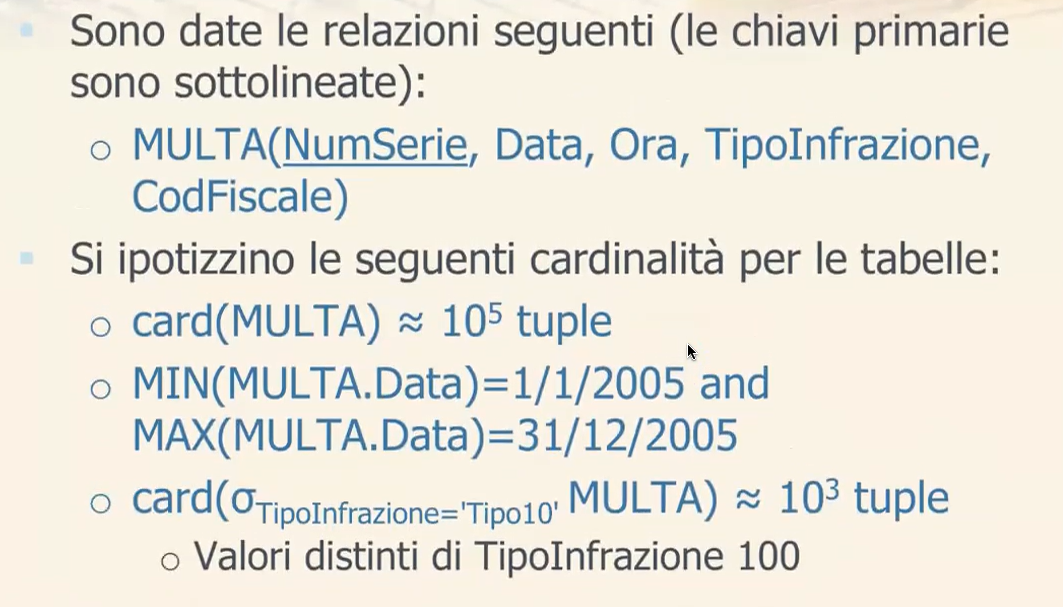
\includegraphics[width=0.8\textwidth]{ex-multa.png}
        \caption{Ex Multa}
        \label{fig:ex-multa}
    \end{figure}
    
\begin{lstlisting}[language=sql]
select data, count(*)
from multa
where data >= 1/10/2005 and data <= 30/11/2005
group by data;
\end{lstlisting}

60 tuple; select statement
\[ \pi_{data, count(*)} \]
60 tuple; hash gb
\[ gb_{data} \]
selettvit\`a $2/12$, card = $2\cdot 10^{4}$
\[ \sigma_{data \geqslant  1/10/2005 \& data \leqslant 30/11/2005} \]
$10^{5}$ tuple, full table scan + filter
\[ multa \]

    Indice su data:
    \begin{itemize}
        \item predicato poco selettivo $(\frac{1}{6})$;
        \item aiuta la gb (dati ordinati rispetto a data);
        \item indice coprente;
        \item indice secondario;
    \end{itemize}
\begin{lstlisting}[language=sql]
create index myindex1 on multa(data);
\end{lstlisting}

    SOLUZIONE 1:
    \begin{itemize}
        \item select statement;
        \item gb hash;
        \item fast full index scan on myindex1
    \end{itemize}

    SOLUZIONE 2:
    \begin{itemize}
        \item select statement;
        \item gb no sort;
        \item full index scan on myindex1 or index range scan on myindex1;
    \end{itemize}

\end{example}

\begin{example}{}{}
\begin{lstlisting}[language=sql]
selct data, count(*)
from multa
where data > = 1/10/2005 and data < = 30/11/2005
    and tipoInfrazione = 'tipo10'
group by data;
\end{lstlisting} 
    QUERY TREE:
    \begin{itemize}
        \item $\pi_{data, count(*)}$
            \begin{itemize}
                \item 60
                \item select statement;
            \end{itemize}
        \item gb data;
            \begin{itemize}
                \item 60
                \item gb sort
            \end{itemize}
        \item $\sigma_{data}$;
            \begin{itemize}
                \item $\frac{1}{6} 10^{3}$
            \end{itemize}
        \item $\sigma_{tipoinfrazione}$;
            \begin{itemize}
                \item $10^{3}$
            \end{itemize}
        \item multa
            \begin{itemize}
                \item $10^{5}$
                \item full table scan + filter
            \end{itemize}
    \end{itemize}


    Indice su data (\emph{non conveniente}):
    \begin{itemize}
        \item bassa selettivit\`a;
        \item poco aiuto a gb (pochi record);
        \item richiede accesso alla tabella per attributo \texttt{tipoInfrazione};
    \end{itemize}
    Indice su tipo infrazione:
    \begin{itemize}
        \item selettivit\`a molto buona $\frac{1}{100}$;
        \item non aiuta gb (per\`o i dati sono pochi);
        \item accesso alla tabella (si ma solo $10^{3}$ tuple);
    \end{itemize}

    SOLUZIONE 1 (indice su tipoInfrazione):
\begin{lstlisting}[language=sql]
create index myindex2 on multa(tipoInfrazione);
\end{lstlisting}
    PIANO DI ESECUZIONE:
    \begin{itemize}
        \item select statement;
        \item gb sort;
        \item access by rowid;
        \item index range scan on myindex2;
    \end{itemize}

    SOLUZIONE 2 (indice coprente):
\begin{lstlisting}[language=sql]
create index myindex3 on multa(tipoInfrazione, data);
\end{lstlisting}
    \texttt{tipoInfrazione} va per primo perch\`e \`e l'attributo pi\`u selettivo.
    
    PIANO DI ESECUZIONE:
    \begin{itemize}
        \item select statement;
        \item gb sort;
        \item fast full index scan on myindex3(i data sono $10^{5}$, si devono ordinare solo 100 record);
    \end{itemize}
\end{example}



\begin{example}{}{}
    \begin{figure}[H]
        \centering
        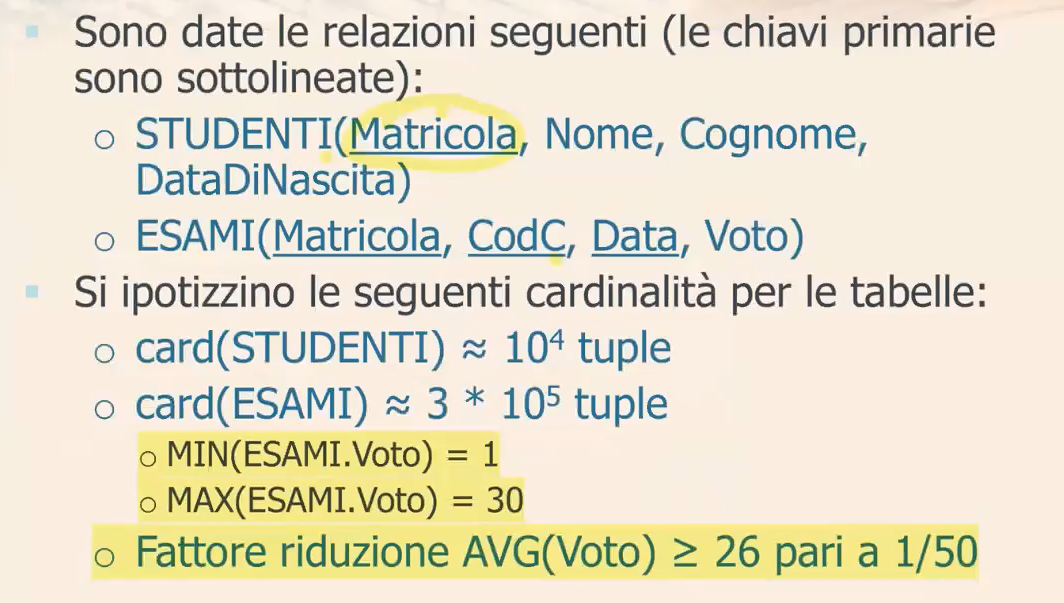
\includegraphics[width=0.8\textwidth]{ex-studenti.png}
        \caption{Ex Studenti}
        \label{fig:ex-studenti}
    \end{figure}

\begin{lstlisting}[language=sql]
select e.matricaola, name, avg(voto)
from esami e, studenti s
where e.matricola = s.matricola and voto >= 18
grop by e.matricola, nome
having avg(voto) >= 26
order by e.matricola;
\end{lstlisting}
    
   QUERY TREE: \\
   $\pi_{matricola,nome,avg(voto)}$ $sort$ $\sigma_{avg(voto) \geqslant  26} $  $ gb_{matricola,nome} ( \sigma_{voto \geqslant 18}(esami)$ $\bowtie_{matricola}$ $studenti )$
\end{example}






\subsection{Concurrency Control}
Grazie al concurrency control si cerca di massimizzare il throughput del numero di transazioni. I sistemi della gestione concorrente sono gestite da uno scheduler, che riceve operazioni di lettura e scrittura. Esistono una serie di problemi di concorrenza, detti \textbf{anomalie}:
\begin{itemize}
    \item \textbf{lost update}: (bot = begin of transaction)
        \begin{figure}[H]
            \centering
            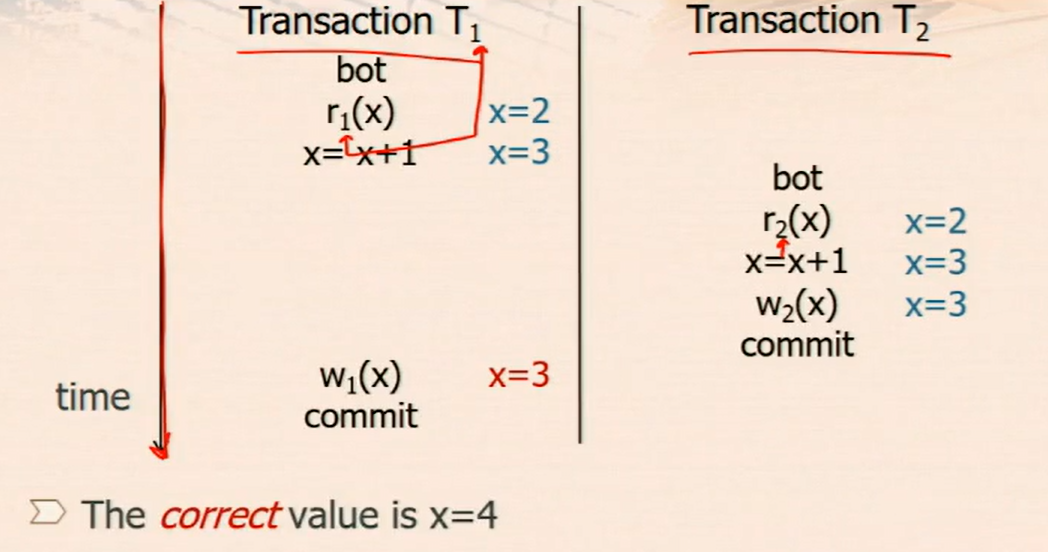
\includegraphics[width=0.8\textwidth]{lost-update.png}
            \caption{Lost Update}
            \label{fig:lost-update}
        \end{figure}
    \item \textbf{dirty read}:
        \begin{figure}[H]
            \centering
            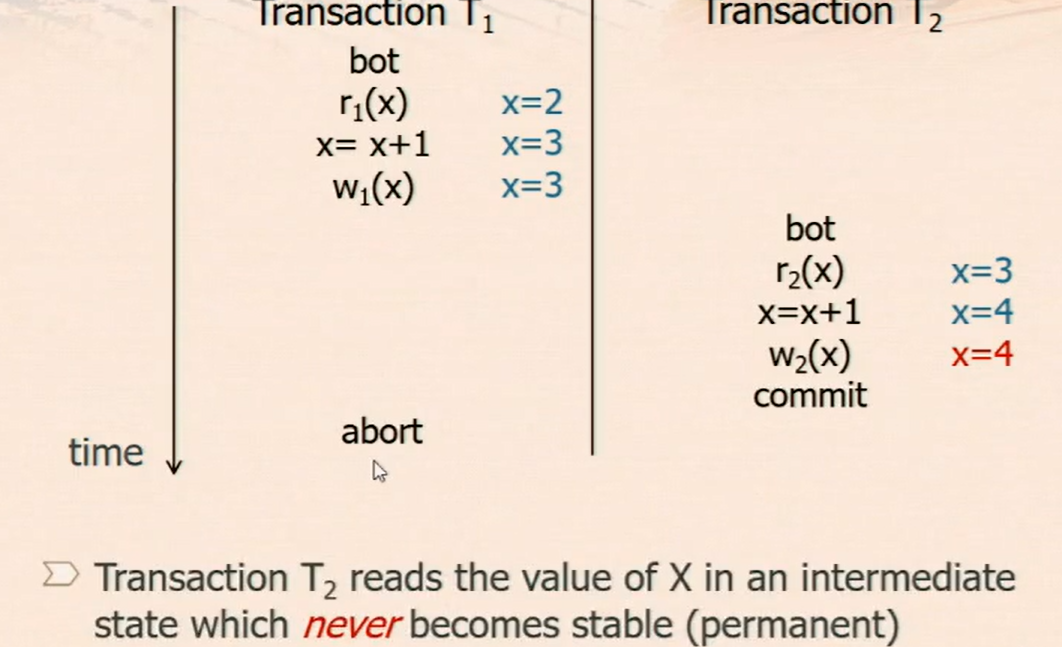
\includegraphics[width=0.8\textwidth]{dirty-read.png}
            \caption{Dirty Read}
            \label{fig:dirty-read}
        \end{figure}
    \item \textbf{inconsistent read}:
        \begin{figure}[H]
            \centering
            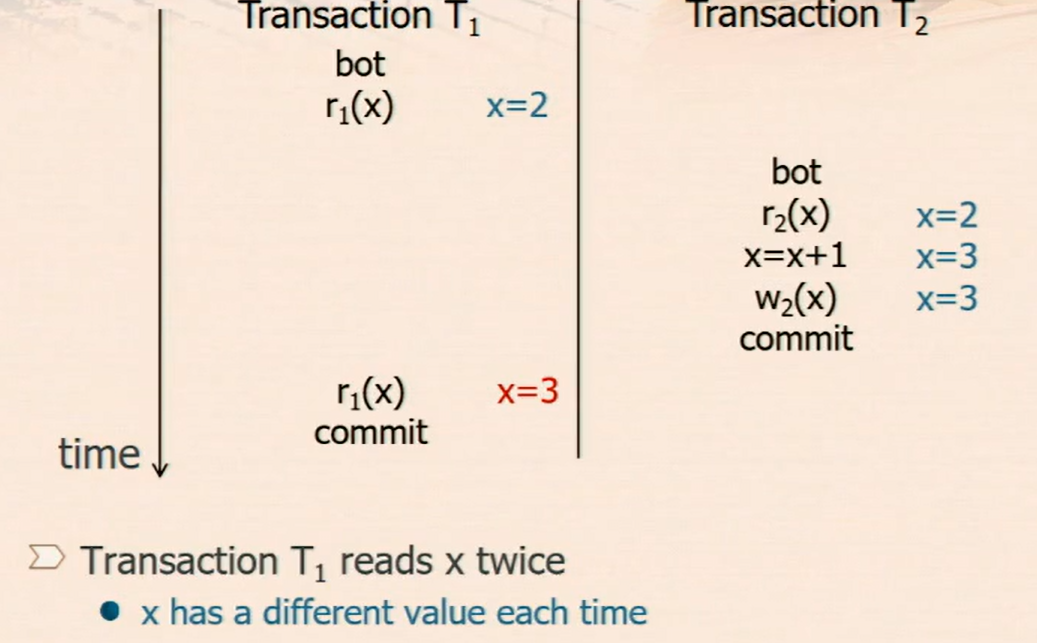
\includegraphics[width=0.8\textwidth]{inconsisten-read.png}
            \caption{Inconsisten Read}
            \label{fig:inconsisten-read}
        \end{figure}
    \item \textbf{ghost update (a)}:
        \begin{figure}[H]
            \centering
            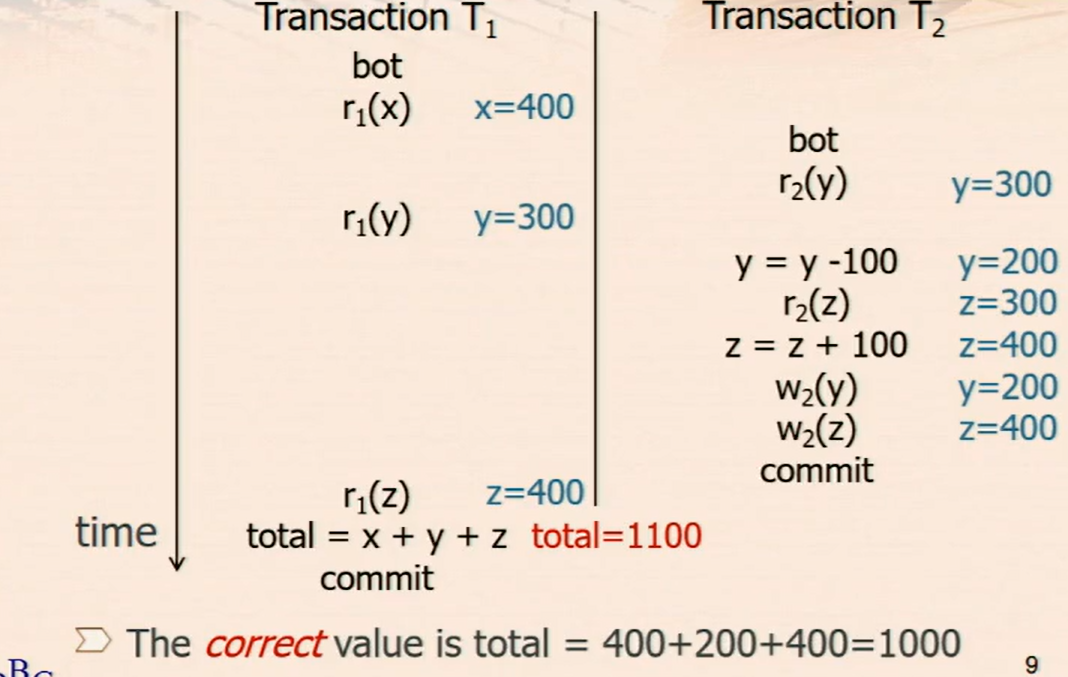
\includegraphics[width=0.8\textwidth]{ghost-read.png}
            \caption{Ghost Read}
            \label{fig:ghost-read}
        \end{figure}
    \item \textbf{ghost update (b)}: come di tipo (a) per\`o viene usato un costrutto aggregato in lettura;
\end{itemize}
Lo schedurel deve decidere se la schedulazione che arriva potrebbe causare dei problemi, per il momento rimuoviamo il problema del dirty read (l'ipotesi \`e che tutte le transazioni vanno a boun fine).

Si parla di \textbf{schedule seriale}, quando le transazioni vengono eseguite fino alla fine, senza mescolare operazioni di transazioni diverse. Si pu\`o dimostrare che quando uno schedule con delle operazione intercalate \`e equivalente ad uno schedule seriale, allore si dice che questo schedule \`e \textbf{serializzabile}. Per avere uno scheduler efficente non si cerca ricostruire in modo perfetto uno scheduling ma il problama viene diviso in classi di equivalenza. Esistono diverse classi di equivalenza:
\begin{itemize}
    \item \textbf{view equivalance}
    \item \textbf{conflict equivalence}
    \item \textbf{2 phase locking}
\end{itemize}


\subsubsection{View Equivalance}
In questo caso vengono definiti due insiemi, \textbf{reads-from}, si ha una lettura $r_i(x)$ preceduta da $w_j(x)$, e nessun altra scrittura in mezzo, ed un isnsime \textbf{final write}, sono le ultime scritture che avvengono sui dati, dopo non vengono pi\`u scritte; si dice che due schedule sono \textbf{equivalenti} se hanno gli stessi set, se lo schedule seriale \`e equivalente allo schedule intercalato allora si dice che \`e \textbf{view serializable}. Questa classe di equivalenze riconosce il lost update, l'inconsistence read ed il ghost update (a). Questo problema \`e di classe NP, il motivo \`e che si devono provare tutti gli ordinamenti, roccogliendo una classe molto ampia di casistiche.


\subsubsection{Conflict Equivalance}
Per questa tipologia di equivalanza vanno definite le azioni conflittutali \textbf{appartengono a transazioni diverse} e \textbf{operano sulla stesso dato}, le azioni sono:
\begin{itemize}
    \item read-write/write-read;
    \item write-write;
\end{itemize}
\begin{figure}[H]
    \centering
    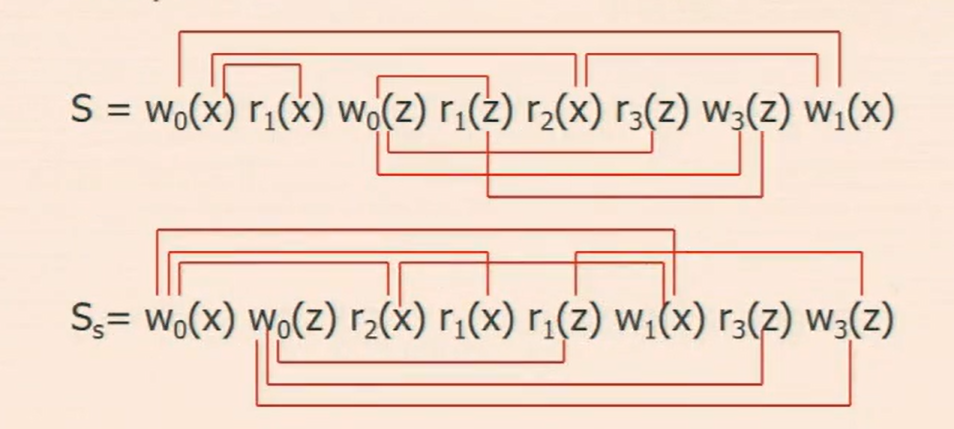
\includegraphics[width=0.8\textwidth]{conflict-equivalance.png}
    \caption{Conflict Equivalance}
    \label{fig:conflict-equivalance}
\end{figure}
Per migliorare questo metodo si utilizza un \textbf{grafo dei conflitti}, ogni nodo rappresenta una transazione, si mette un arco orientato per ogni conflitto che si trova, se il grafo dei conflitti \`e aciclico allora lo schedule \textbf{conflict serializable}, altrimenti no.
\begin{figure}[H]
    \centering
    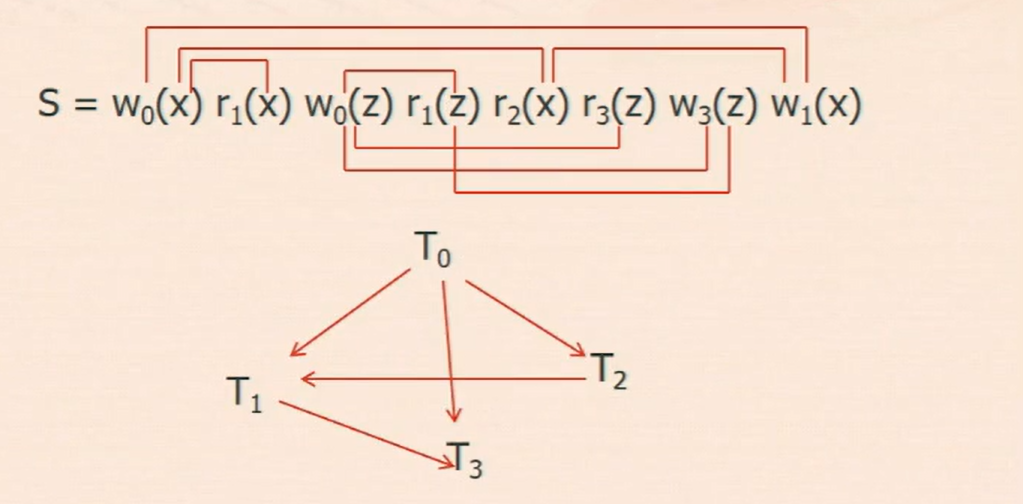
\includegraphics[width=0.8\textwidth]{grafo-dei-conflitti.png}
    \caption{Grafo Dei Conflitti}
    \label{fig:grafo-dei-conflitti}
\end{figure}


\subsubsection{2 Phase Locking}
Qusto metodo \`e molto utilizzata, si utilizza un \textbf{lock}, questo lock viene usato per le letture e per le scritture. I lock sono condivisi dalle transazioni. Lo scheduler diventa in questa situazione un \textbf{lock manager} decidento se tolgiere o dare dei lock in base allo stato del sistema, una volta che la transazione riceve il lock allora pu\`o accedere alla pagina, altrimenti aspetta il rilascio del lock in possesso di un altra transazione. Il lock manager guarda una tabella dei lock per decidere quale lock dare e la tabella dei conflitti, dove vengono salvate le richieste.

Il lock manager controlla il valore dei lock per decidere cosa fare qundo una transazione ne richede uno. Nei db si utilizzano i \textbf{2 phase lockgin}, esiste una prima fase detta \textbf{growing phase}, dove si acquisiscono i lock, ed una fase detta \textbf{shrinking phase}, questo si inizia a rilasciare i lock non \`e pi\`u possibile acquisirne di nuovi fino allo svuotarsi completo.

Su utilizziamo il \textbf{strict 2 phase locking}, ovvero abilitare il drop dei lock solo dopo il commit o l'abort di un transazione, si risolve anche il problema del \textbf{dirty read}.

Le primitivi di lock sono:
\begin{itemize}
    \item \texttt{R-lock(T, x, ErrorCode, TimeOut)};
    \item \texttt{W-lock(T, x, ErrorCode, TimeOut)};
    \item \texttt{UnLock(T, x)};
\end{itemize}
Un transazione chiede un lock, il db controlla la tabella dei conflitti, se \`e disponibile allora il lock gli viene assegnato, se la richiesta non pu\`o essere soddisfatta, allora la transazione viene messa in una coda, sar\`a ripescata quando la risorsa sar\`a disponibile.


\subsubsection{Locking Gerarchico}
Si pu\`o decidere la granuralit\`a del locking:
\begin{itemize}
    \item l'intera tabella;
    \item gruppi di tuple (frammenti);
    \item l'intera pagina;
    \item la singola tupla;
    \item il singolo attributo;
\end{itemize}
\begin{figure}[H]
    \centering
    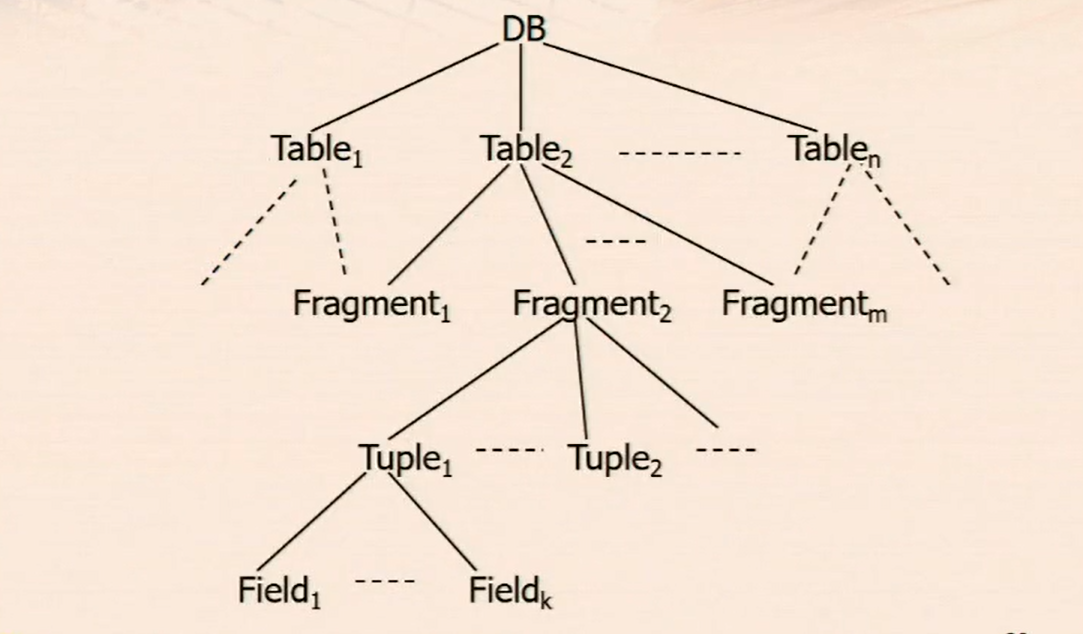
\includegraphics[width=0.8\textwidth]{gerarchia-dei-lock.png}
    \caption{Gerarchia Dei Lock}
    \label{fig:gerarchia-dei-lock}
\end{figure}
Per creare questo tipo di lock vengono prese le primitivi dei lock con in aggiunta una \textbf{intenzione}.
\begin{itemize}
    \item Shared Lock (SL) = Read Lock;
    \item Exclusive Lock (XL) = Write Lock;
\end{itemize}

I lock vengono assegnati a partire dalla radice dell'albero, mentre vengono rilasciati dalle foglie, se si vuole richiedere un SL (Shared Lock) o un ISL (Intention SL) su un nodo, una transazione devo possedere un ISL o un IXL (Intention Exlusive Lock) del nodo padre.
\begin{figure}[H]
    \centering
    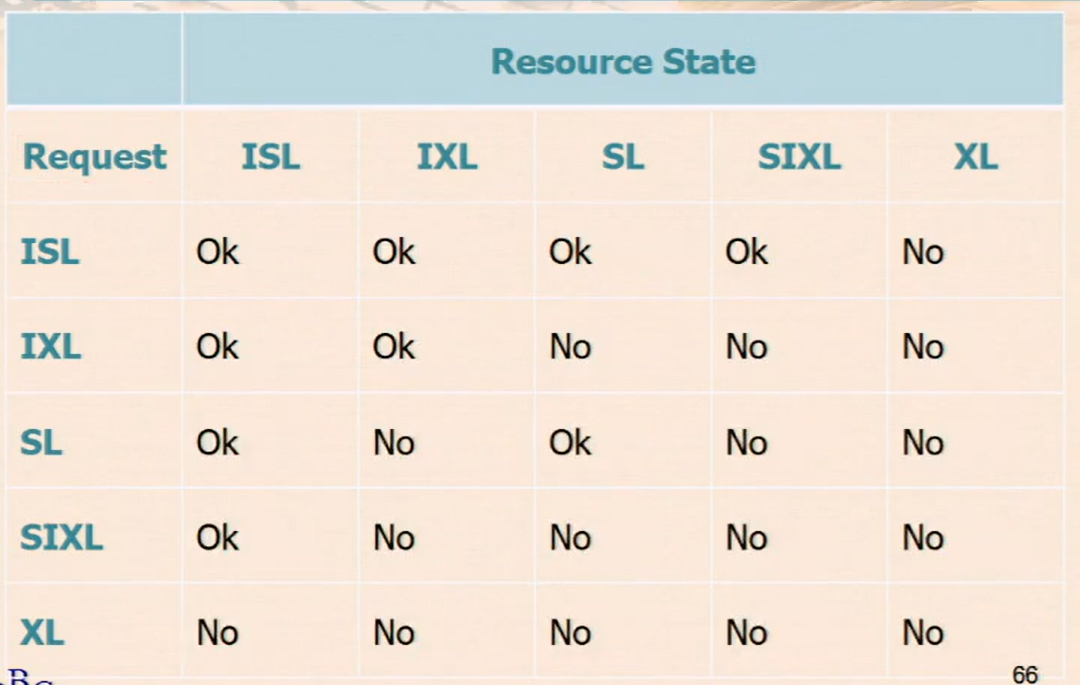
\includegraphics[width=0.8\textwidth]{compatibility-matric.png}
    \caption{Compatibility Matric}
    \label{fig:compatibility-matric}
\end{figure}


\subsubsection{Predicate Locking}
Il 2 phase locking non riesce a bloccare il ghost update (b), il predicate locking risolve questo problema \textbf{mettendo un lock sulle tuple che soddifano un predicato}. Solitamnte \`e presente un indice per quel predicato, ed il problema del predicate locking bloccando proprio l'indice, in questo modo non viene bloccata l'intera tabella.


\subsubsection{Locking in SQL}
In sql si possono definire i tipi di transazione:
\begin{itemize}
    \item read-write (default);
    \item read only;
    \item livelli di isolamento;
\end{itemize}
I livelli di isolamento sono:
\begin{itemize}
    \item \textbf{serializable}: include il predicate locking;
    \item \textbf{reapeatable read}: strict 2pl;
    \item \textbf{read committed}: non pi\`u 2pl, i lock in scrittura vengono rilasciati dopo il commit;
    \item \textbf{read uncommitted}: non 2pl, si legge senza acquisire il lock;
\end{itemize}
La sintassi \`e:
\begin{lstlisting}[language=sql]
set transaction
[isolation level <isolation_level>]
[read only]
[read write]
\end{lstlisting}


\subsubsection{Deadlock}
Per risolvere con certezza il problema del deadlock \`e l'uso di un timeout, alla termine di questo timeout la transazione viene uccisa. Un modo di prevenire il deadlock \`e il \textbf{2pl pessimistico}, ovvero richiedere a priori tutti i lock di cui la transazoine ha bisogno, un altro metodo \`e l'\textbf{analisi del timestamp}, quando due transazioni richiede un lock si da la precedenza alla transazioni pi\`u giovani. Si pu\`o anche utilizzare un \textbf{grafo delle attese} (se \`e ciclico c'\`e un deadlock), solitamnte viene utilizzato in pochi casi di db distribuiti, il motivo \`e che questa tecnica \`e molto costosa.



\subsection{Reliability Manager}
La gestione dall'affidabilit\`a garantisce due propriet\`a, l'\textbf{atomicit\`a} e la \textbf{durabilit\`a}. Il manager deve gestire delle letture e scritture ulteriori per garantire la correttezza delle operazione fatte sul db, queste informazioni sono contenute nei \textbf{file di log}, che si trovano nella \textbf{memoria stabile}. La memoria stabile si tratta di un memoria che non pu\`o subire guasti (non realistico), questo si ottiene con della ridondanza, supponiamo che i guasti del db non hanno effetto sulla memoria stabile.

I log sono dei file sequenziali che registrano le attivit\`a delle transazioni, scritti in modo efficiente. Esistono dei delimitatori delle transazioni:
\begin{itemize}
    \item \textbf{begin} B(T);
    \item \textbf{commit} C(T);
    \item \textbf{abort} A(T);
\end{itemize}
Le modificazioni sono (O = object, AS = after state, BS = before state):
\begin{itemize}
    \item insert I(T,O,AS);
    \item delete D(T,O,BS);
    \item update U(T,O,BS,AS);
\end{itemize}
Fare \textbf{UNDO} di un oggetto, vuol dire rimuover quell'oggetto della base dati, il \textbf{REDO} \`e rifare l'azione sull'oggetto. Su questa operazioni deve valere la propriet\`a di \textbf{idempotenza}:
\[ undo(undo(action)) = undo(action) \]
Il gestore richiede il \textbf{checkpoint}, il cui unico obbiettivo \`e quello di velocizzare l'operazione di recovery, ovvere il punto in cui viene scirtto il db.

Il \textbf{DUMP} crea una copia fisica dell'intero db, quando si termina l'operazione si scrive nei log, e dal quel punto \`e possibile fare un recovery in caso di guasti.

Esistono dei protocolli per la gestione del log:
\begin{itemize}
    \item \textbf{Write Ahead Log} (WAL), \`e un protocollo che prima di scrivere sul db tutta l'informazione viene prima scritta nel log il BS, e poi viene fatta l'operazione.
    \item \textbf{Commit Precedence}, prima di fare commit si scrive prima valore dell'AS e poi viene fatto il commit.
\end{itemize}
Per questi due protocolli il BS e l'AS vengono scritti insieme. Il log viene scritto in modo \textbf{sincrono} quando un pagina viene scaricata su disco (force) o quando viene fatto un commit, in modo \textbf{asincrono} quando si fa un dump del db. Se nei log non si trova il record del commit (in caso di guasto), la transazione deve essere ripetuta.

A fronte di guasto, che possono essere di \textbf{sistema} (sistema operativo) o \textbf{media} (supporti fisici). Esiste il modello del \textbf{fail-stop}, quando si cerca di fare del recovery, viene continuato a fare fino a quando non si \`e sicuri di avere dei dati consistenti.
\begin{figure}[H]
    \centering
    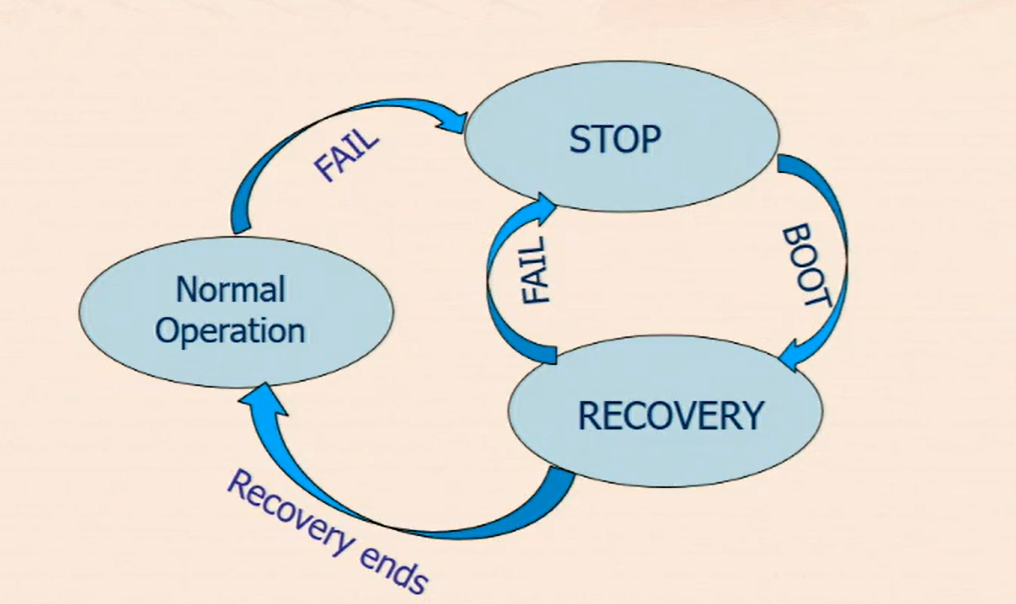
\includegraphics[width=0.8\textwidth]{fail-stop.png}
    \caption{Fail Stop}
    \label{fig:fail-stop}
\end{figure}
Esistono due tipi di restart:
\begin{itemize}
    \item \textbf{warm restart}: system failure;
    \item \textbf{cold restart}: media failure;
\end{itemize}

\subsubsection{Warm restart}
\begin{figure}[H]
    \centering
    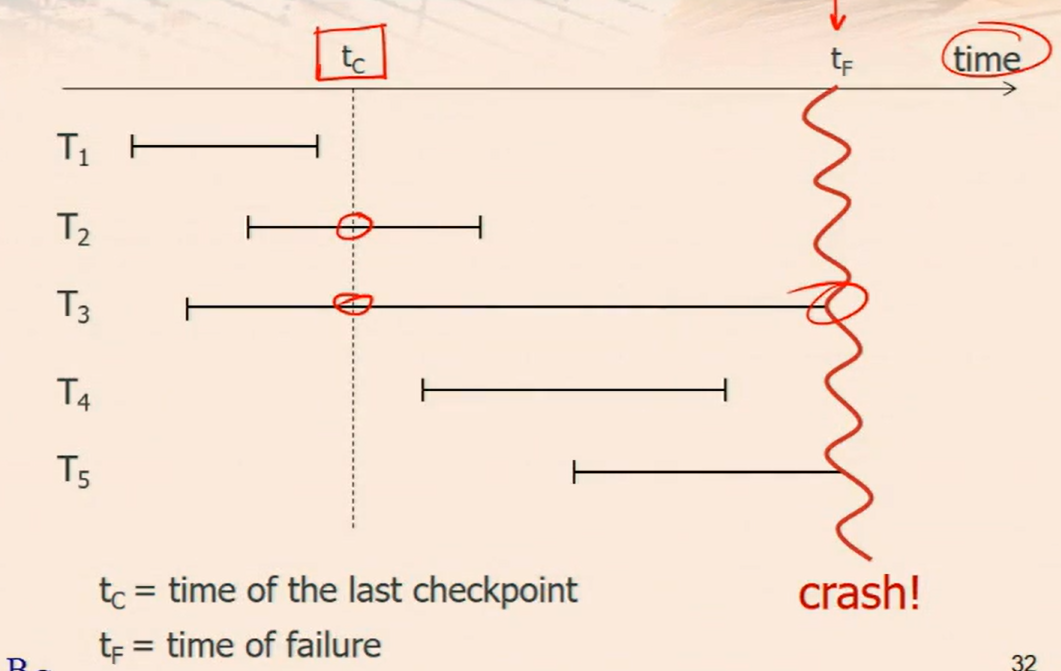
\includegraphics[width=0.8\textwidth]{warm-restart.png}
    \caption{Warm Restart}
    \label{fig:warm-restart}
\end{figure}
In questo caso:
\begin{itemize}
    \item 1: non bisogno di operazioni di recovery;
    \item 2, 4: hanno bisogno di redo;
    \item 3, 5: hanno bisogno di undo;
\end{itemize}
L'algoritmo di ripristino funziona nel segutne modo:
\begin{enumerate}
    \item legge il log al contrario e cerca il checkpoint pi\`u recente;
    \item inizia a cercare le transazioni da cui fare undo e redo;
    \item crea due liste per undo e redo e mette nella lista di undo tutte le transazoini trovate che si trovano nel checkpoint;
    \item legge il log dal checkpoint fino all'ultimo log e per ogni commit che trova sposta la transazione dall lista di undo alla lista di redo, e per ogni begin che trovo sposta la lista nella lista degli undo;
    \item si parte dall'ultima entra e percorrendo il log si fanno tutte le azioni di undo;
    \item si parte dall'operazione pi\`u vecchia di tutte le transazioni presenti nella lista dei redo e andando in avanti si fanno tutte le operazioni di redo;
\end{enumerate}


\subsubsection{Cold Restart}
Una parte del db \`e andato perduto per un guasto fisico, di parte dall'ultimo record di dump e si fanno tutte le operazioni transazionionali presenti nel log e al termine si fa un warm restart per ripristinare lo stato consistente dei dati.





\newpage
\section{DBMS Distribuiti}
L'obbiettivo dei db distribuiti \`e quello di distribuire dati e computazione su macchine diverse. I vari tipi di architettura possono essere:
\begin{itemize}
    \item client/server;
    \item database distribuito, ogni db \`e indipendente, le proprit\`a acid devono essere valide anche con i dati distribuiti;
    \item db replicati, detti server di replicazione;
    \item architetture parallele;
\end{itemize}
Nello scenario dei db distribuiti si ha la situazione in cui un client potrebbe acedere a pi\`u nodi, ed ogni nodo opera in maniera indipendetne. Distribuire i dati permette di  avere una localizzazione, maggior disponibilit\`a di dati e maggiore scalabilit\`a, oltre a risolver il prblema di single point of failure.

I dati possono essere frammentati tra i diversi db, pu\`o avvinere a livello di tabella come proiezione, selezione, o un mix. Quando si applica una selezione per ricostruire la tabella basta un operazione di unione. Se si frammenta a in modo verticale la chiave primaria deve essere necessariamente aggiunta, per ricostruire la tabella basta fare un join. Quando si decide di frammentare la relazione, la tabella orinale non esister\`a pi\`u ma sar\`a possibiel ricostruirla opportunamente attraverso degli schema, ognuno di questi frammenti sar\`a gestito in modo indipendente da ogni db su cui si trova. Avere dei dati frammentati permette di avere una ridondanza dei dati, avendo un costo maggiore per operazioni di aggiornamento.

Esistono vari livelli di trasparenza per i frammenti quando si scrivono delle query sql per sapere da dove prendere i dati:
\begin{itemize}
    \item \textbf{fragmentation transparency}: la query viene scritta come se la tabella su un unico db;
    \item \textbf{allocation transparency}: la query viene scritta essendo a conoscenza dei frammenti, senza sapere per\`o su quele server si trovano;
    \item \textbf{language transparency}: la query viene scritta richiedendo i dati da un server specifico;
\end{itemize}
Le transazioni possono essere classificate.
\begin{itemize}
    \item \textbf{remote request}: solo lettura;
    \item \textbf{remote transaction}: eseguire un comando qualunque si un singolo server;
    \item \textbf{distributed transaction}: si esegue qualsisi comando sql, ogni comando \`e riferito ad un singolo nodo, in questo caso la gestione delle transazione deve essere pi\`u robusto (2 phase commit);
    \item \textbf{distibuted request}: ogni comando pu\`o far riferimento a dati distribuiti su server diversi, mi garantisce la trasparenza di frammentazione;
\end{itemize}



\begin{figure}[H]
    \centering
    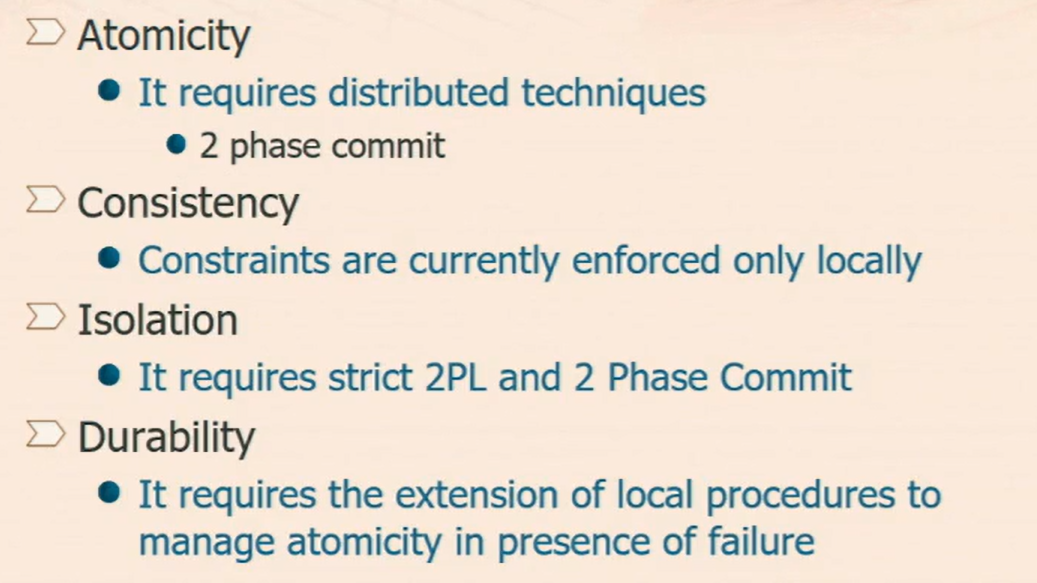
\includegraphics[width=0.8\textwidth]{acid-propreties-in-distributed-dbms.png}
    \caption{Acid Propreties In Distributed Dbms}
    \label{fig:acid-propreties-in-distributed-dbms}
\end{figure}




...



\section{NoSQL}
Le caratteristiche principali sono dei NoSql sono:
\begin{itemize}
    \item nessuna possibilit\`a di fare join;
    \item nessuno schema;
    \item scalabilit\`a orizzontale (aggiungere molte cpu in parallelo);
\end{itemize}
Nei db non-relazionali non esistono tabelle ma documenti, o key-value, graph based, columnar storage.

I tipi di db nosql sono:
\begin{itemize}
    \item \textbf{key-value pair}: sono veloci ed efficenti, tutti i dati vengono messi in cache;
    \item \textbf{column oriented}: simili ai datawarehouse;
    \item \textbf{graph db}: usati quando dei dati hanno delle relazioni tra di loro;
    \item \textbf{documento}: ogni documento possiede degli attributi chiave valore, i documneti possono essere nestati tra di loro;
\end{itemize}

\subsection{CouchDB}
CouchDB (cluster of unrelieable comodity hardware). I punti pricipali dell'architettura di coudchdb sono:
\begin{itemize}
    \item possibilit\`a di fare \textbf{mapreduce}: ogni nodo pu\`o fare in modo distribuito del mapping e del reducing su uno stream di dati;
    \item \textbf{replicazione} dei dati nei vari nodi;
    \item \textbf{distribuzione} del sistema;
    \item interrogazioni attraverso un API HTTP;
\end{itemize}

\subsubsection{MapReduce}
Esempio di mapReduce:
\begin{lstlisting}[language=java]
// Map function
function(doc) {
    key = doc.matricola
    value = [doc.mark, doc.cfu]
    emit(key, value);
}

// Reduce function
function(key, values) {
    S = sum([ X*Y for X,Y in values])
    N = sum([ Y for X,Y in values])
    AVG = S/N
    return AVG;
\end{lstlisting}



\subsubsection{Replication}
Un approccio alla replicazione \`e il \textbf{master-slave}, dove un unico server \`e il master, che prende tutte le scritture e gli update, tutti gli altri nodi sono degli slave, da cui \`e possibile solo leggere i dati, i cambiamenti possono essere propagati in maniera sincrona (simile al 2PC), oppure l'asynchronous replication dove il master fa un commit locale, ogni slave fa il fetch indipendenti dei nuovi dati.


\subsubsection{Distribuzione}
Le caratteristica di un sistema sono:
\begin{itemize}
    \item \textbf{Consistenti};
    \item \textbf{Availability};
    \item \textbf{Partizionamento};
\end{itemize}
Da qui nasci il \textbf{teorema CAP}.
\begin{theorem}{CAP}{cap}
    In ogni istante \`e possibile ottenere solo due caratteristiche contemporaneamente.
\end{theorem}
\begin{itemize}
    \item CA: si ricade nel db singolo;
    \item CP: quando si fa il 2PC;
    \item AP: non ci importa della global consistency;
\end{itemize}
Lo combinazioni possono essere intercambiate in tempi diversi in modo continuo. Infatti nel mondo non relazionale esiste la caratteristica \textbf{BASE}, (al contrario di ACID):
\begin{itemize}
    \item Basically Available;
    \item Soft state;
    \item Eventually consistent;
\end{itemize}
Per la risoluzione dei conflitti si possono utilizzare:
\begin{itemize}
    \item revision: come con il version control, quando si fetcha una revision si prende quella con il numero pi\`u basso e con l'hash ordinato;
    \item 
\end{itemize}


Nel mondo non relazionale non esistono le transazioni, pi\`u operazioni infatti non possono essere rese atomiche, per\`o le operazioni su in singolo documento sono transazionali, quindi un modo di procedere \`e quello di modellare il documento come una transazione.


\subsection{MongoDB}
In MongoDB:
\begin{itemize}
    \item table = collection;
    \item record = document;
    \item column = field;
\end{itemize}
Esempio di query su mongoDB:
\begin{lstlisting}[language=java]
db.<collection name>.find( {<conditions>}, {<fields of interest>});

// mongoDB
db.people.find();

// sql
select *
from people;
\end{lstlisting}
Filtraggio:
\begin{lstlisting}[language=java]
db.people.find({age:55});

db.people.find({}, {user_id: 1, status: 1});

db.people.find({age: {\$gt: 25, \$lte: 50} });

db.people.find({\$or: [{status: "A"}, {age: 55}] });

db.people.find({ status: {\$in: ["A", "B"]} });
\end{lstlisting}
In mongoDB per recuperare altri documenti si possono usare l'\textbf{objectId} ed il \textbf{DBRef}.

Si possono anche usare degli operatori aggreganti con il metodo \texttt{.aggregate()}.
\begin{lstlisting}[language=java]
db.people.aggregate([
  { \$group: {
    _id: null,
    mytotal: { \$sum: "\$age"},
    mycount: { \$sum: 1}
  }
}]);
\end{lstlisting}
Per utilizzare le coordinate spaziali si utilizza GeoJSON:
\begin{lstlisting}[language=java]
{
  _id: "...",
  location: {
    type: "Point",
    coordinates: [
      45.324,   // lat
      52,123    // lng
    ] 
  }
}
\end{lstlisting}
Poi si crea un indice sul campo:
\begin{lstlisting}[language=java]
db.collection.createIndex({location: "2dsphere"});

db.collection.find({location: {
    \$near: {
      type: "Point",
      coordinates: [34.353, 4.535]
    },
    \$maxDistance: 435,
    \$minDistance: 43
  }
});
\end{lstlisting}
I risultati vengono restituti in ordine dal pi\`u vicino al pi\`u lontano.







\end{document}
